\documentclass[supercite,macfont]{HustGSClassPaper}

\classname{研究生课程设计}
\title{基于云的协同机械 CAD 系统设计与实现}
\stunum{待填写}
\author{待填写}
\classnum{待填写}
\instructor{待填写}
\school{待填写}
\date{\today}

\usepackage{xltxtra}
\usepackage{bm}
\usepackage{graphicx}
\usepackage{booktabs}
\usepackage{tabularx}
\usepackage{longtable}
\usepackage{array}
\usepackage{enumitem}

\graphicspath{{figures/}}

\begin{document}
\maketitle

\clearpage
\pagenumbering{Roman}

\begin{cnabstract}{云 CAD；协同设计；Three.js；WebSocket；版本管理；智能辅助建模}
本文围绕《基于云的协同机械 CAD 系统设计与实现》课程设计题目，面向“本地稳定运行、功能链路完整、结构清晰可讲解”的交付目标，设计并实现了一个可用于课程展示与报告提交的协同机械 CAD 最小可交付系统。系统采用 React + TypeScript + Vite 构建前端界面，使用 Three.js 完成三维图形渲染，采用 Zustand 维护建模状态；后端基于 Node.js + Express + WebSocket 实现房间状态维护与实时协同广播；数据层通过本地 JSON 文件完成项目保存与版本快照管理。

系统支持 Box、Cylinder、Sphere 等基础实体建模，支持 Line、Circle、Rectangle 等草图对象表达，并实现了基于 Rectangle 与 Circle 草图的 Extrude 操作。与此同时，系统提供双窗口同房间实时协同、在线用户显示、远端光标同步、Save / Load、版本恢复以及 Undo / Redo 等关键能力。为增强项目的创新性表达，系统增加了 Smart Assist 自然语言辅助建模入口，并在架构层预留了 OpenCASCADE/Wasm、PostgreSQL、OBS 及 AI 辅助设计等后续扩展方向。

实验与联调结果表明，该系统能够在 macOS 本地环境下稳定运行，并较完整地覆盖课程设计考核项中关于架构设计文档、核心功能实现、代码质量、创新性和演示答辩的要求。本文实现强调工程取舍与演示稳定性之间的平衡，在较低实现复杂度下完成了协同 CAD 的核心闭环，为后续演进为更完整的 Web CAD 平台奠定了实现基础。
\end{cnabstract}

\begin{enabstract}{Cloud CAD; collaborative design; Three.js; WebSocket; version management; smart-assisted modeling}
This report presents the design and implementation of a cloud-based collaborative mechanical CAD system for a graduate course project. Instead of targeting a full industrial-grade CAD kernel, the project focuses on building a stable, locally runnable, and presentation-ready minimum viable product. The frontend is implemented with React, TypeScript, and Vite, while Three.js is used for 3D rendering and Zustand is used for state management. The backend is built with Node.js, Express, and WebSocket to maintain room state and broadcast collaborative operations. Project persistence and version snapshots are implemented with local JSON files.

The system supports primitive modeling with Box, Cylinder, and Sphere, basic sketch objects such as Line, Circle, and Rectangle, and an Extrude feature that converts Rectangle or Circle sketches into 3D entities. It also provides real-time collaborative editing across multiple browser windows, online user presence, remote cursor indicators, Save / Load, version restore, and Undo / Redo. To strengthen the innovation aspect, a lightweight Smart Assist natural-language command entry is introduced, while the architecture keeps extension points for OpenCASCADE/Wasm, PostgreSQL, object storage, and AI-assisted design.

The implementation and verification results show that the system is suitable for local demonstration, report writing, and oral defense. It covers the major grading dimensions of architecture documentation, core functionality, code quality, innovation, and presentation readiness, while remaining structurally clear and extensible.
\end{enabstract}

\tableofcontents[pagenum=true]

\clearpage
\pagenumbering{arabic}

\section{引言}

\subsection{研究背景}

机械 CAD 系统是现代工程设计与制造流程中的关键工具，在零件建模、结构设计、工艺分析与工程表达等方面发挥着重要作用。传统机械 CAD 软件通常以单机桌面形态为主，虽然功能强大，但也存在若干局限：

\begin{itemize}[leftmargin=2em]
  \item 多用户协同能力有限，难以满足分布式团队实时共同编辑的需求；
  \item 软件部署和运行环境相对复杂，不利于轻量化演示与教学；
  \item 工业级几何内核集成复杂，在课程设计周期内难以完成完整实现。
\end{itemize}

随着浏览器渲染能力提升、WebSocket 实时通信机制普及，以及云协同编辑技术的发展，基于 Web 的协同 CAD 系统成为具有工程实践价值的研究方向。React、Three.js、Node.js 等技术栈为构建轻量化云协同 CAD 提供了可行基础\cite{react2025,threejs2025,nodejs2025}。

\subsection{研究目标}

本课程设计并不以替代工业级 CAD 软件为目标，而是以“稳定演示、顺利提交、便于讲解、可持续扩展”为优先原则，完成一个云协同机械 CAD 最小可交付系统（MVP）。本项目的具体目标包括：

\begin{enumerate}[leftmargin=2em]
  \item 设计并实现一个本地可运行的 CAD 主界面；
  \item 支持基础建模、草图表达、拉伸成型等核心功能；
  \item 支持双窗口同房间实时协同编辑；
  \item 支持保存、加载、版本快照与恢复；
  \item 保持代码结构清晰，并为后续扩展预留接口。
\end{enumerate}

\section{需求分析}

\subsection{功能需求}

根据题目要求和课程设计的演示场景，系统需要满足以下功能需求：

\begin{enumerate}[leftmargin=2em]
  \item \textbf{前端 CAD 界面}：包含 Ribbon 风格工具栏、Feature Tree、Three.js 三维视图区、属性面板、房间状态与在线用户区域；
  \item \textbf{基础建模能力}：支持 Box、Cylinder、Sphere；支持 Line、Circle、Rectangle 草图对象；支持基于 Rectangle / Circle 的 Extrude；
  \item \textbf{协同能力}：支持房间机制、多人实时同步、在线用户列表与远端光标显示；
  \item \textbf{存储能力}：支持 Save / Load、版本快照、版本恢复；
  \item \textbf{操作控制}：支持 Undo / Redo；
  \item \textbf{创新入口}：支持 Smart Assist 自然语言辅助建模。
\end{enumerate}

\subsection{非功能需求}

除功能实现外，本项目还需满足以下非功能需求：

\begin{itemize}[leftmargin=2em]
  \item 本地运行稳定，不依赖 Docker；
  \item 不要求远程部署，优先适配 macOS 本地开发环境；
  \item 系统结构清晰，便于课程报告与答辩讲解；
  \item 对 OpenCASCADE/Wasm、数据库和对象存储保留扩展空间。
\end{itemize}

\section{系统总体设计}

\subsection{技术栈选型}

本系统的主要技术栈如下：

\begin{itemize}[leftmargin=2em]
  \item 前端：React + TypeScript + Vite；
  \item 三维渲染：Three.js；
  \item 状态管理：Zustand；
  \item 后端：Node.js + Express + ws；
  \item 数据存储：本地 JSON 文件。
\end{itemize}

选型原因如下：

\begin{itemize}[leftmargin=2em]
  \item React 与 TypeScript 适合构建结构清晰的组件化界面；
  \item Three.js 能够高效实现基础三维几何体与交互视图；
  \item WebSocket 适合房间协同与操作广播；
  \item JSON 文件存储实现简单、调试方便、部署门槛低；
  \item 整体技术栈能够满足课程设计“本地稳定可演示”的目标。
\end{itemize}

\subsection{架构思想}

本系统采用“前端重计算、后端轻协同”的架构思想，即：

\begin{itemize}[leftmargin=2em]
  \item 前端负责对象创建、参数编辑、Three.js 渲染、Undo / Redo 等；
  \item 后端负责房间状态维护、协同消息广播、保存与版本管理；
  \item 数据层负责当前房间状态和历史版本快照的持久化。
\end{itemize}

这种设计降低了后端复杂度，使系统更适合课程设计周期与本地运行环境，同时也保留了后续引入几何内核的升级路径。

\section{系统架构设计}

\subsection{总体架构}

系统总体由前端 CAD 客户端、后端协同服务和本地存储层组成。前端与后端通过 HTTP 与 WebSocket 两种方式通信：HTTP 用于获取状态、保存项目和恢复版本，WebSocket 用于实时协同广播。

\begin{generalfig}[htb]{系统总体架构图}{fig:arch}
  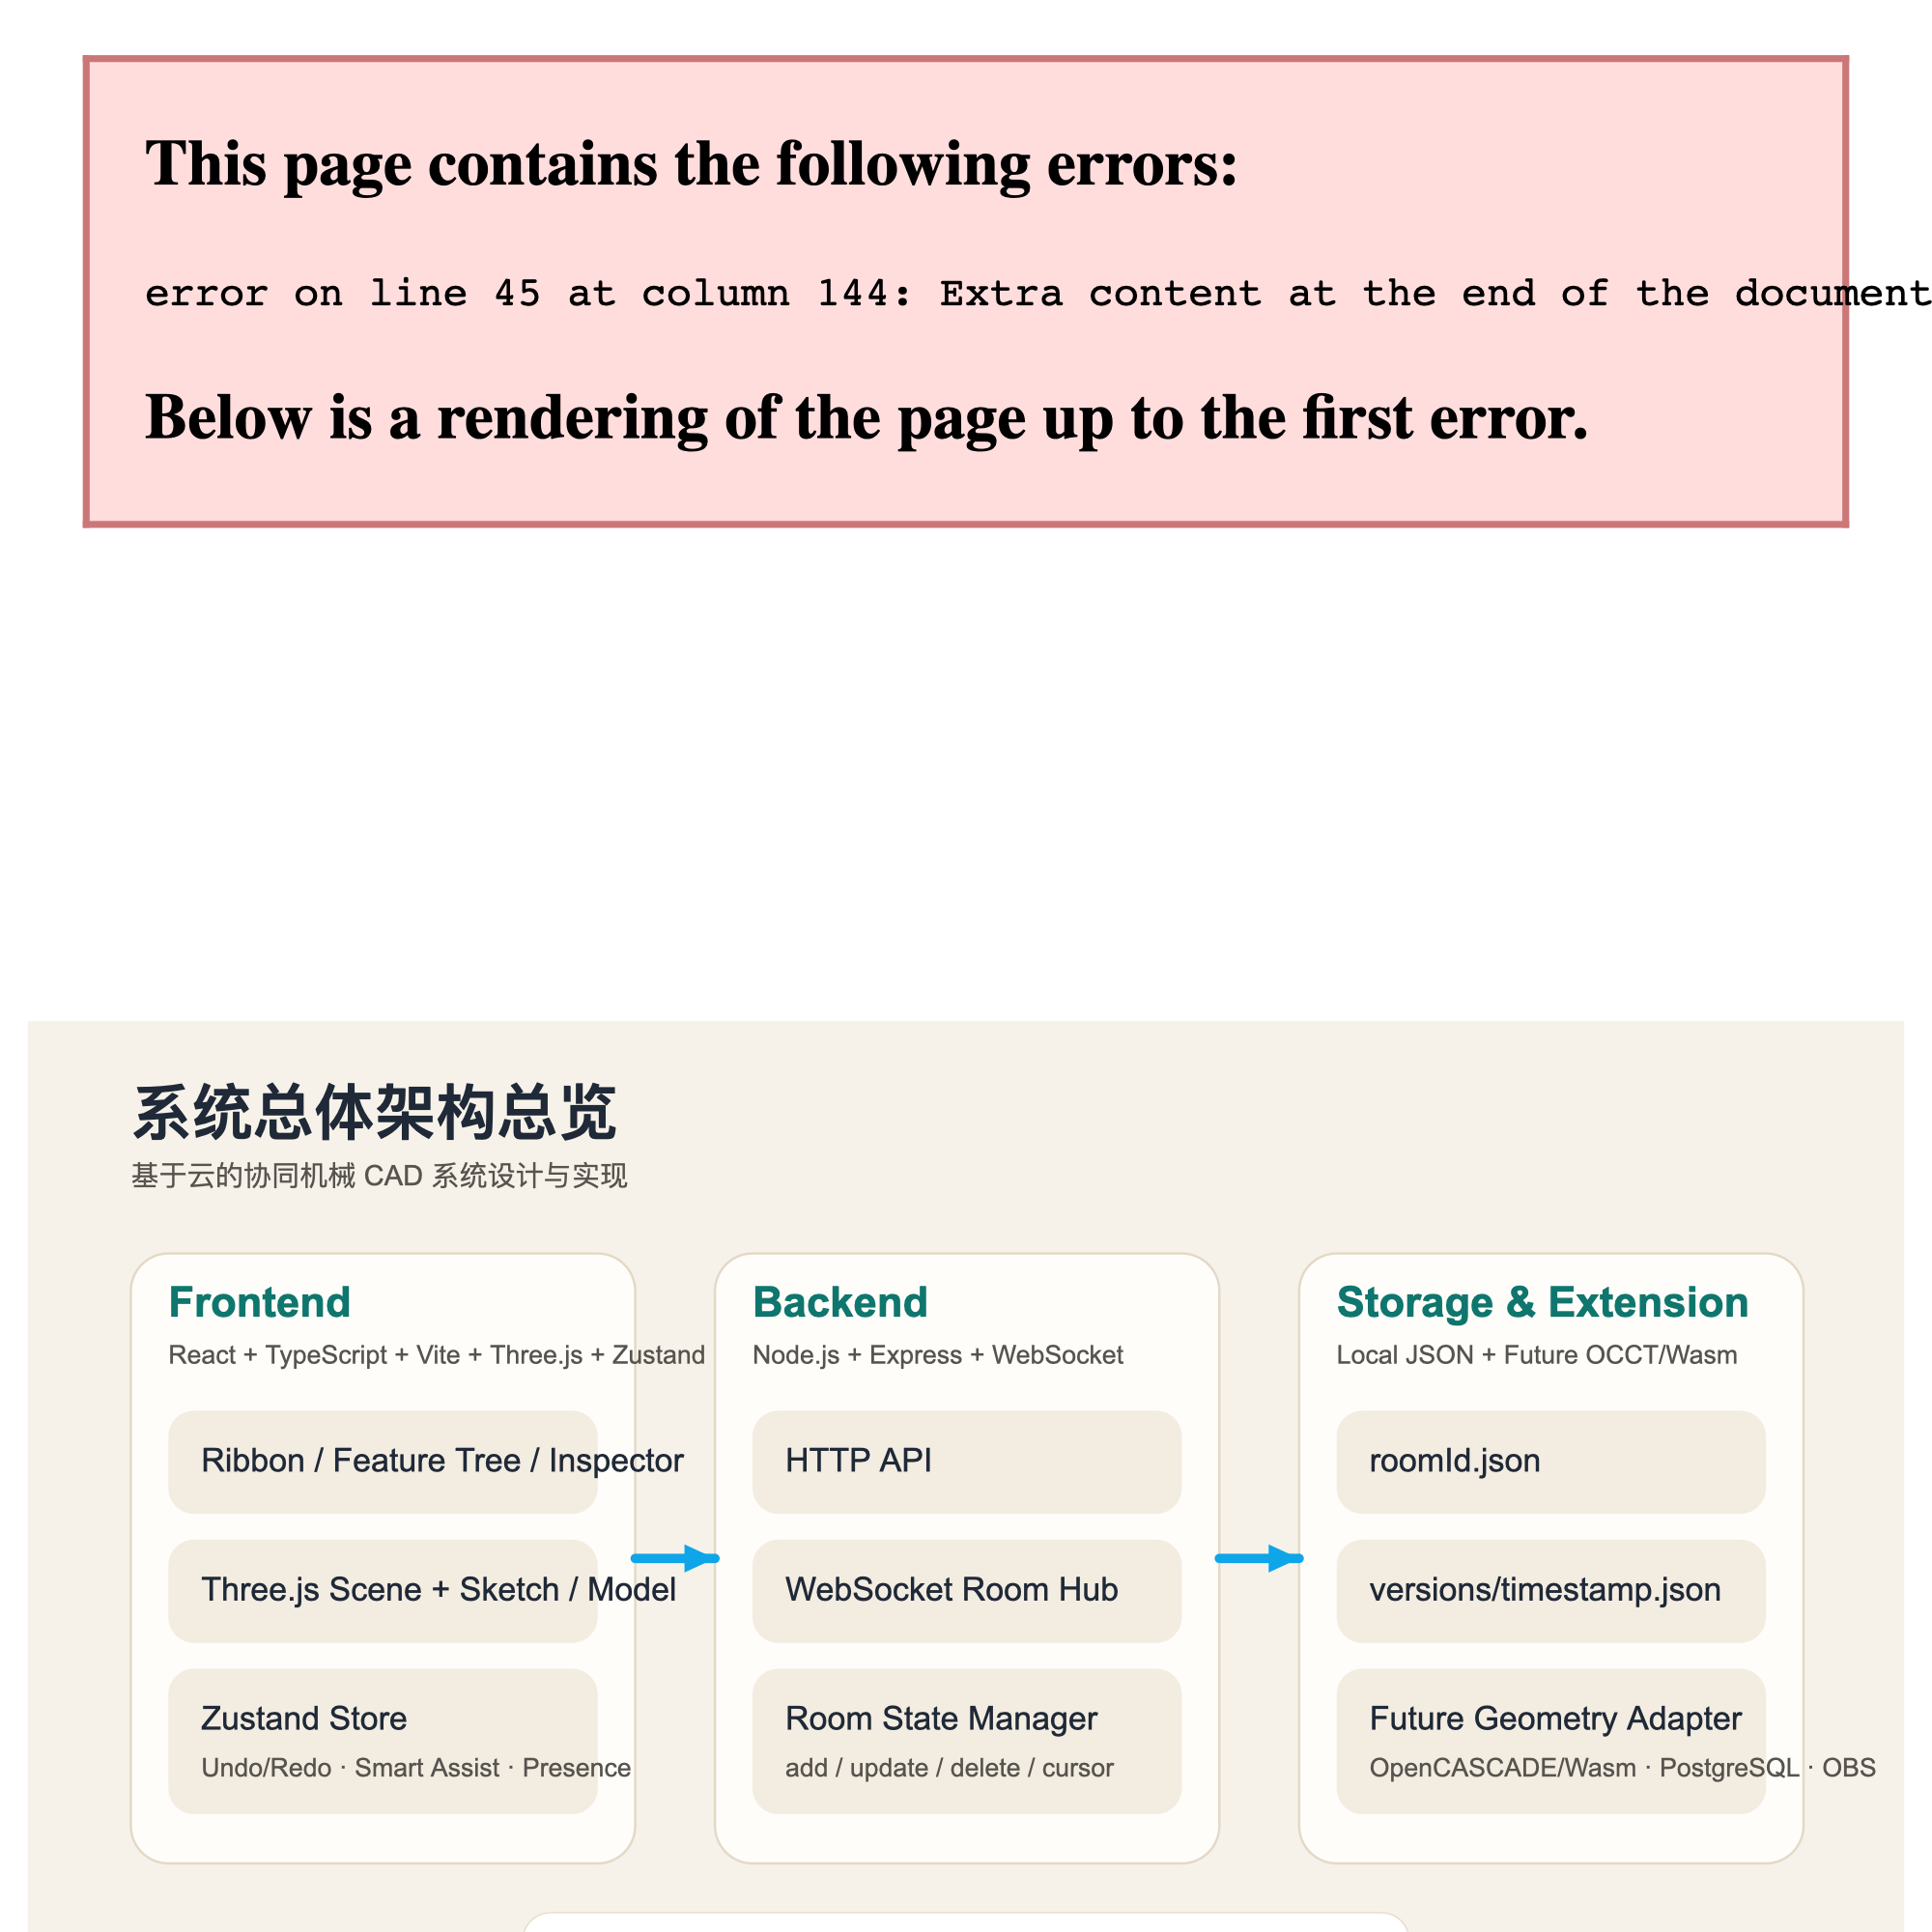
\includegraphics[width=\textwidth]{architecture-overview.png}
\end{generalfig}

如\autoref{fig:arch}所示，前端负责建模与渲染，后端负责协同与状态维护，存储层负责房间 JSON 与版本快照。

\subsection{模块关系 UML}

为便于从软件工程角度说明系统边界，本文进一步给出前后端核心模块关系 UML 图，如\autoref{fig:uml}所示。可以看到，前端以 \texttt{CadStore} 作为状态中枢，负责连接工具栏、对象树、属性面板与三维视图；后端则以 \texttt{Server}、\texttt{RoomManager} 和 \texttt{Storage} 形成清晰的协同与持久化分层。

\begin{generalfig}[htb]{系统模块关系 UML 图}{fig:uml}
  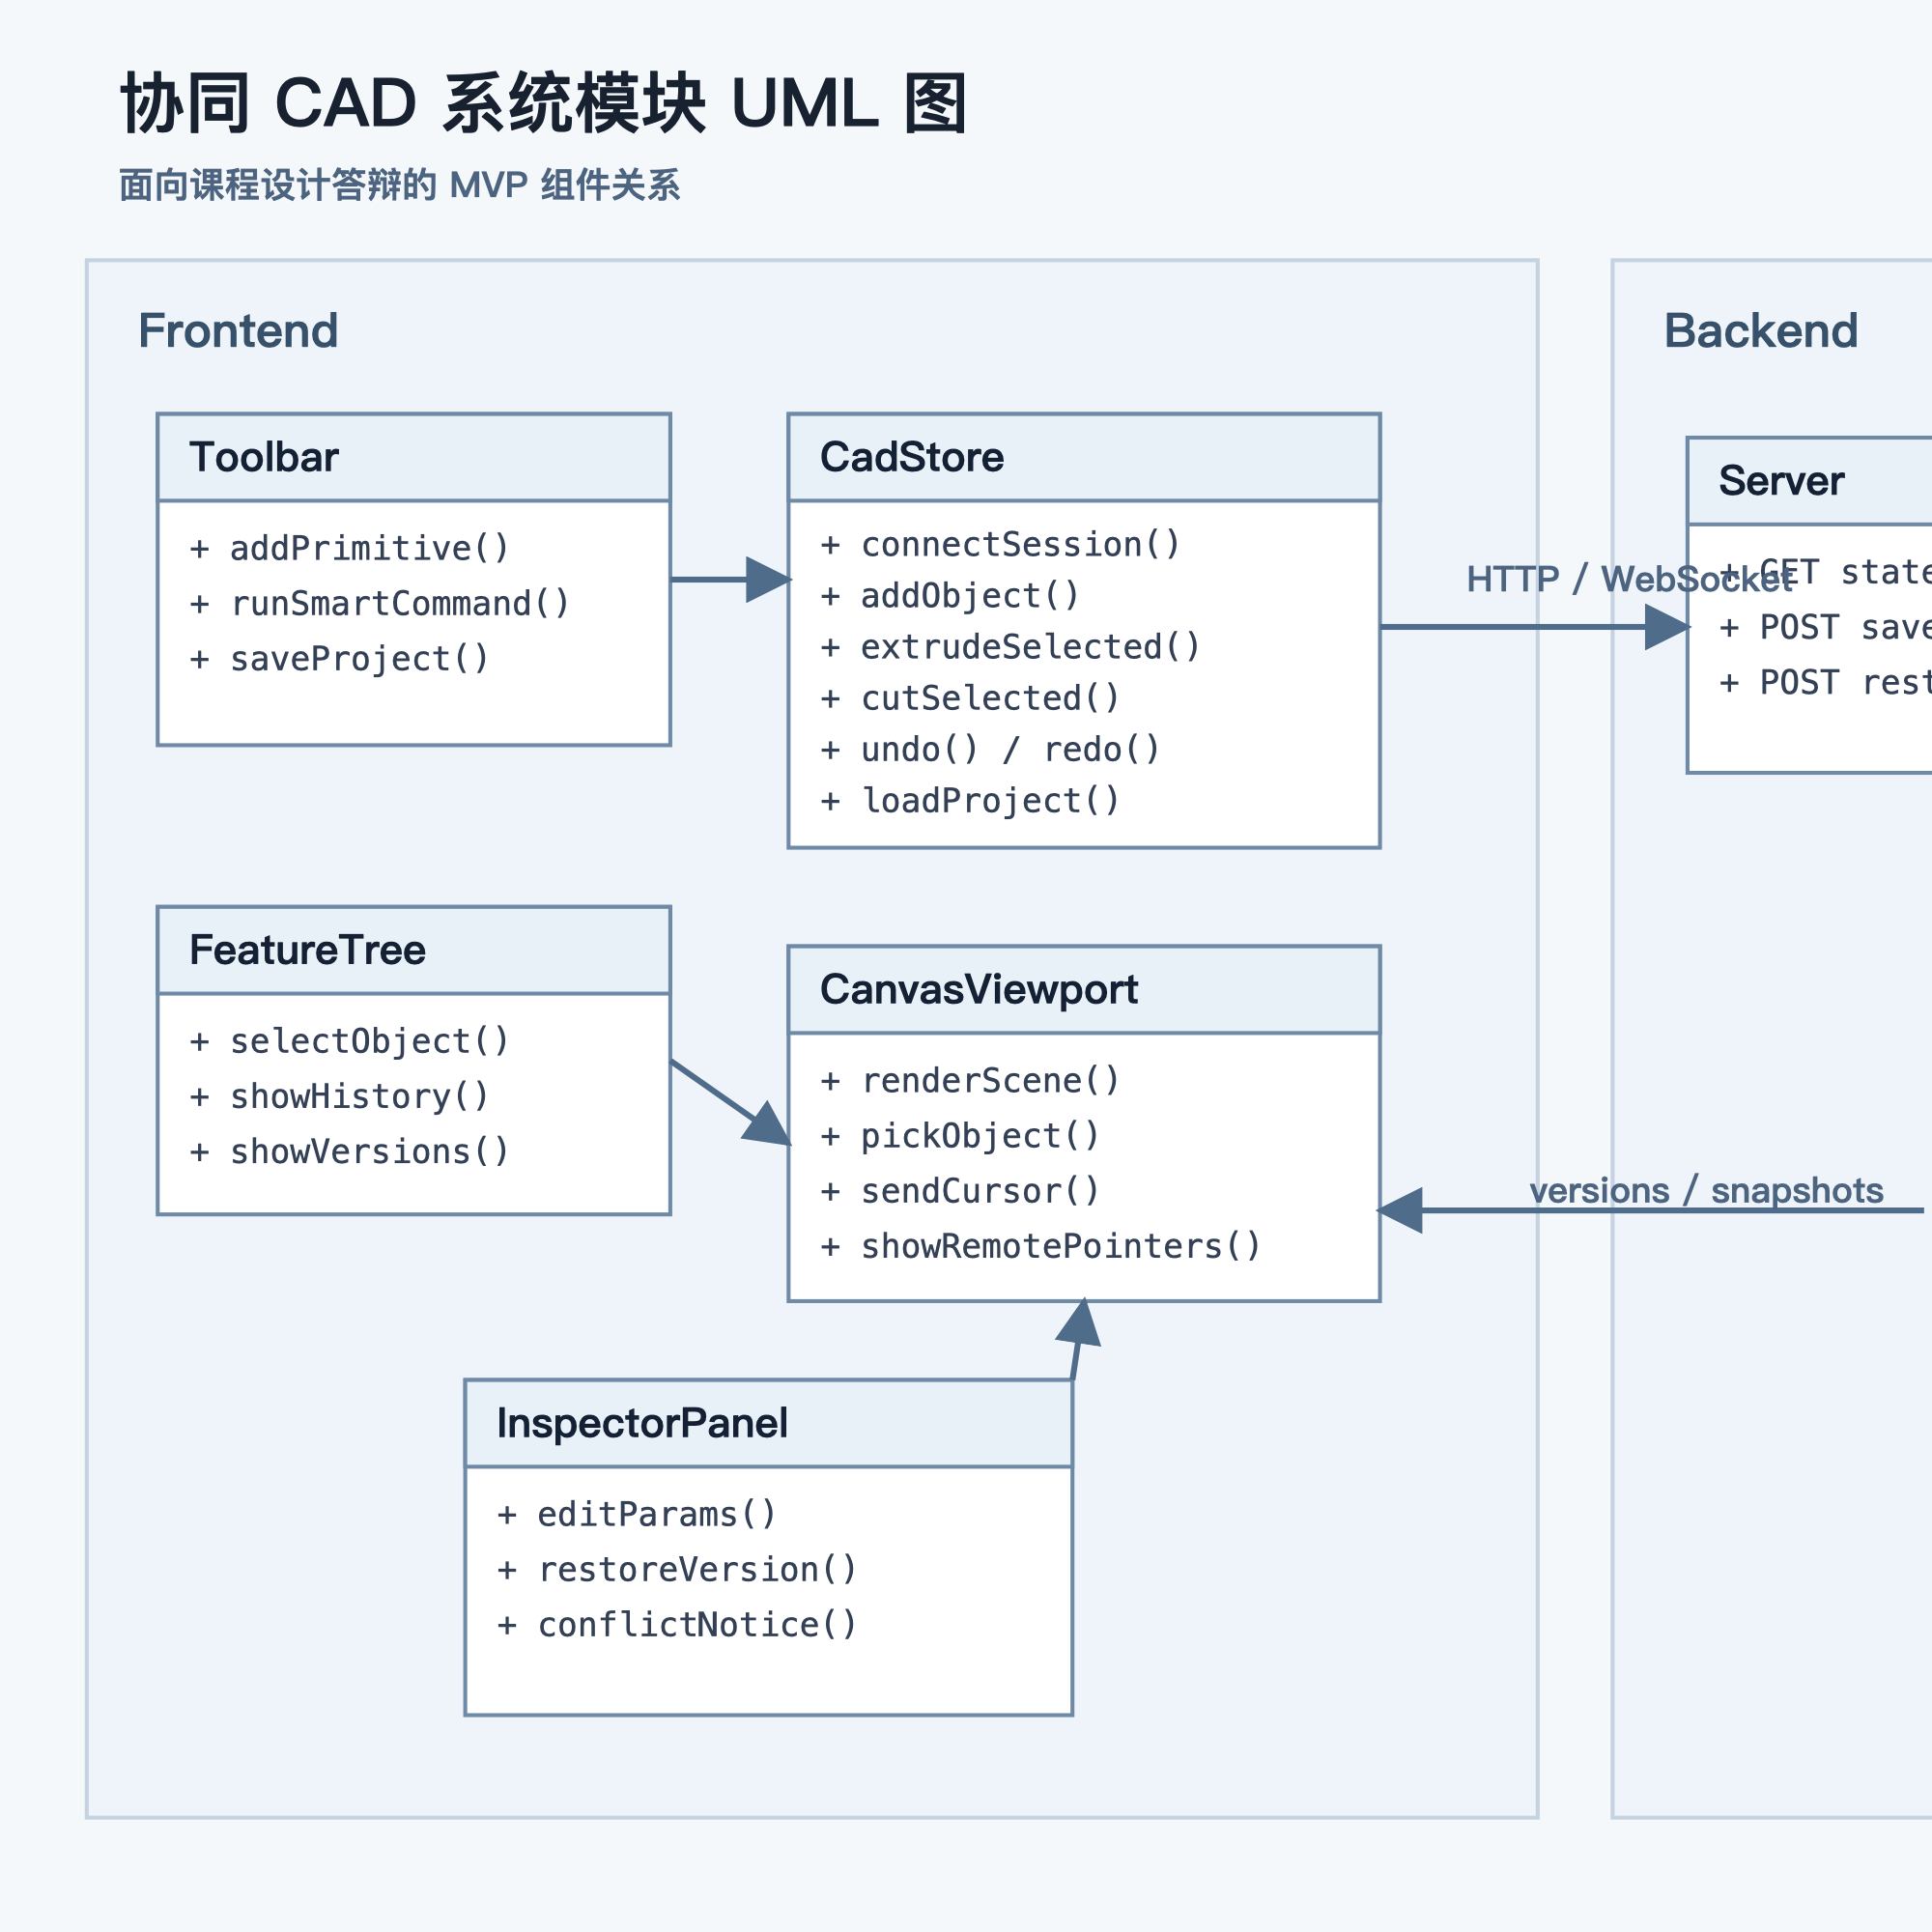
\includegraphics[width=\textwidth]{module-uml.png}
\end{generalfig}

\subsection{前端模块设计}

前端主要模块包括：

\begin{itemize}[leftmargin=2em]
  \item \texttt{Toolbar}：用于触发建模、保存、加载、智能命令；
  \item \texttt{FeatureTree}：显示建模历史与对象列表；
  \item \texttt{CanvasViewport}：负责 Three.js 场景渲染与拾取；
  \item \texttt{InspectorPanel}：编辑当前对象参数与恢复版本；
  \item \texttt{StatusPanel}：展示房间 ID、在线用户、连接状态；
  \item \texttt{useCadStore}：统一管理前端状态与协同逻辑。
\end{itemize}

\subsection{后端模块设计}

后端模块包括：

\begin{itemize}[leftmargin=2em]
  \item \texttt{server.ts}：Express API 与 WebSocket Server 入口；
  \item \texttt{room-manager.ts}：房间状态维护、操作应用、在线用户与光标管理；
  \item \texttt{storage.ts}：JSON 保存、版本快照、版本恢复；
  \item \texttt{types.ts}：房间状态、消息类型和对象结构定义。
\end{itemize}

\subsection{数据流设计}

系统的数据流可概括为：

\begin{enumerate}[leftmargin=2em]
  \item 用户输入用户名和房间号；
  \item 前端通过 WebSocket 加入房间；
  \item 用户执行建模操作，前端先本地更新；
  \item 前端发送操作消息到后端；
  \item 后端更新房间状态并广播到其他客户端；
  \item 用户点击 Save 时，后端写入 JSON 并生成版本快照。
\end{enumerate}

\begin{generalfig}[htb]{实时协同与持久化数据流图}{fig:dataflow}
  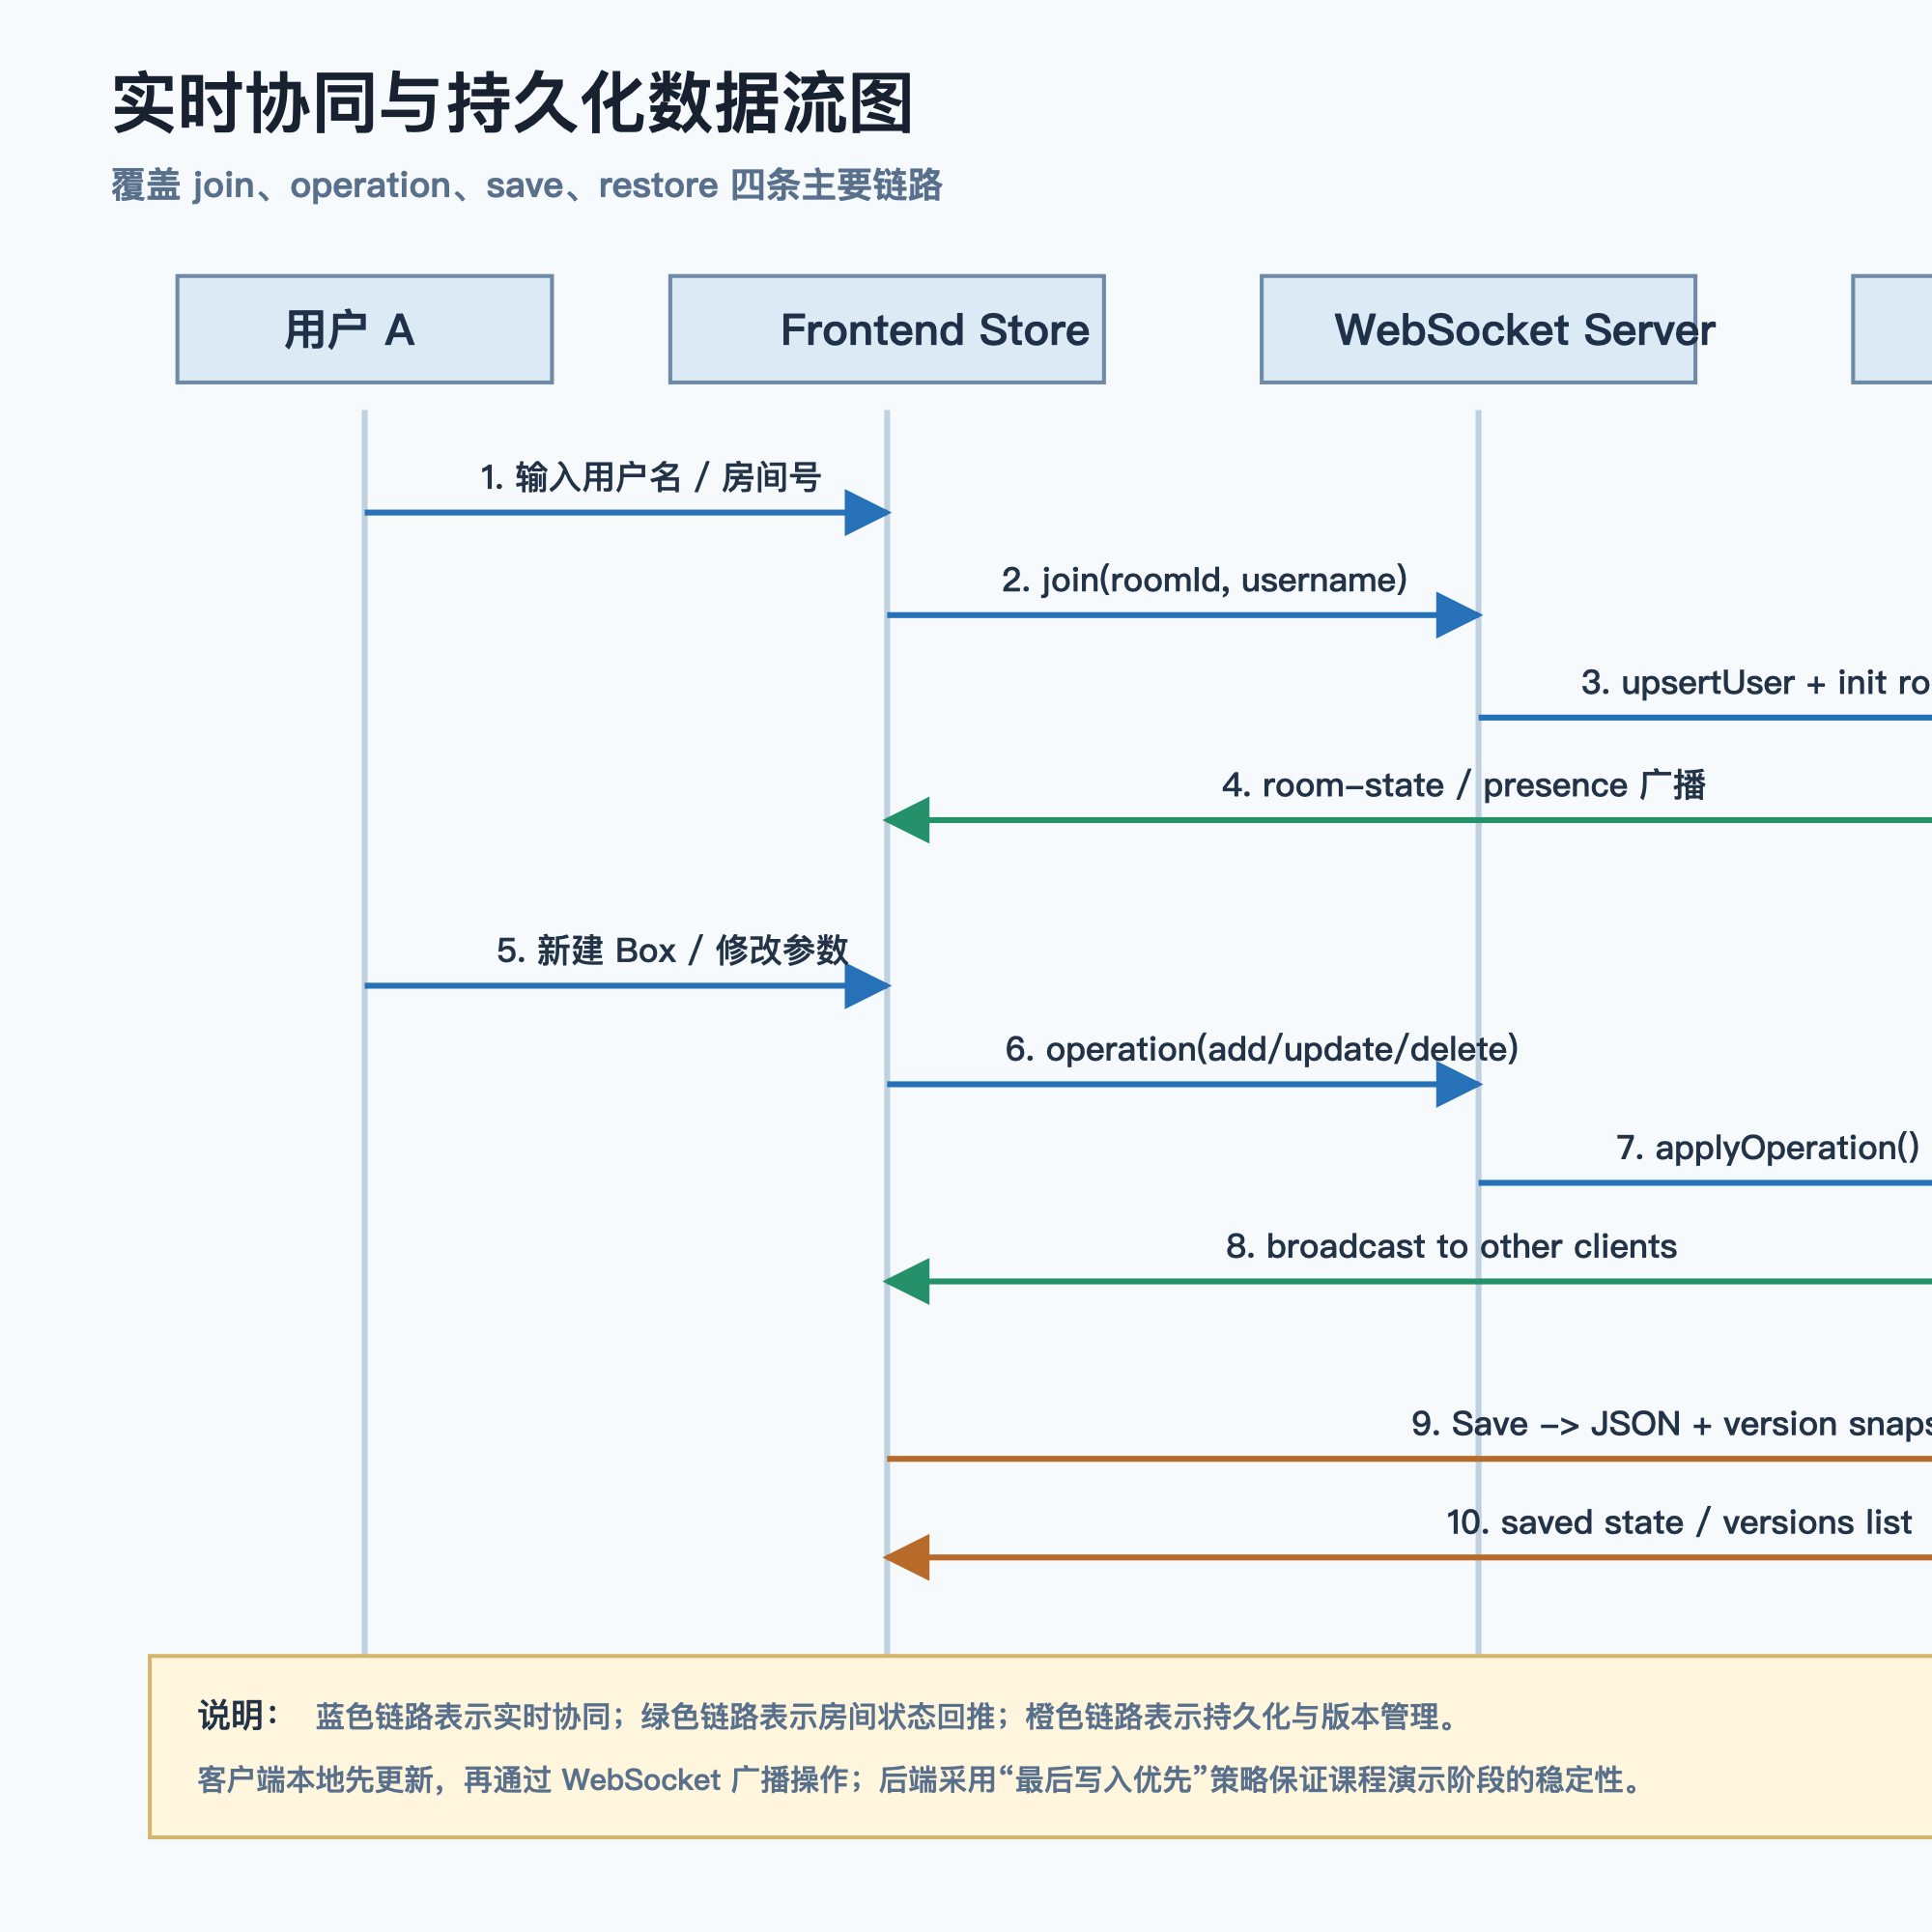
\includegraphics[width=\textwidth]{collab-dataflow.png}
\end{generalfig}

\subsection{OpenCASCADE / Wasm 扩展预留}

考虑到课程设计周期和本地稳定演示要求，当前系统没有直接集成 OpenCASCADE/Wasm，而是将其作为后续扩展方向进行架构预留。如\autoref{fig:wasm}所示，未来可在前端增加 \texttt{Geometry Adapter} 和浏览器 Worker 中的 OCCT Wasm 模块，将高层特征命令转换为更强的 B-Rep 求解与布尔运算流程。

\begin{generalfig}[htb]{OpenCASCADE / Wasm 预留通信机制图}{fig:wasm}
  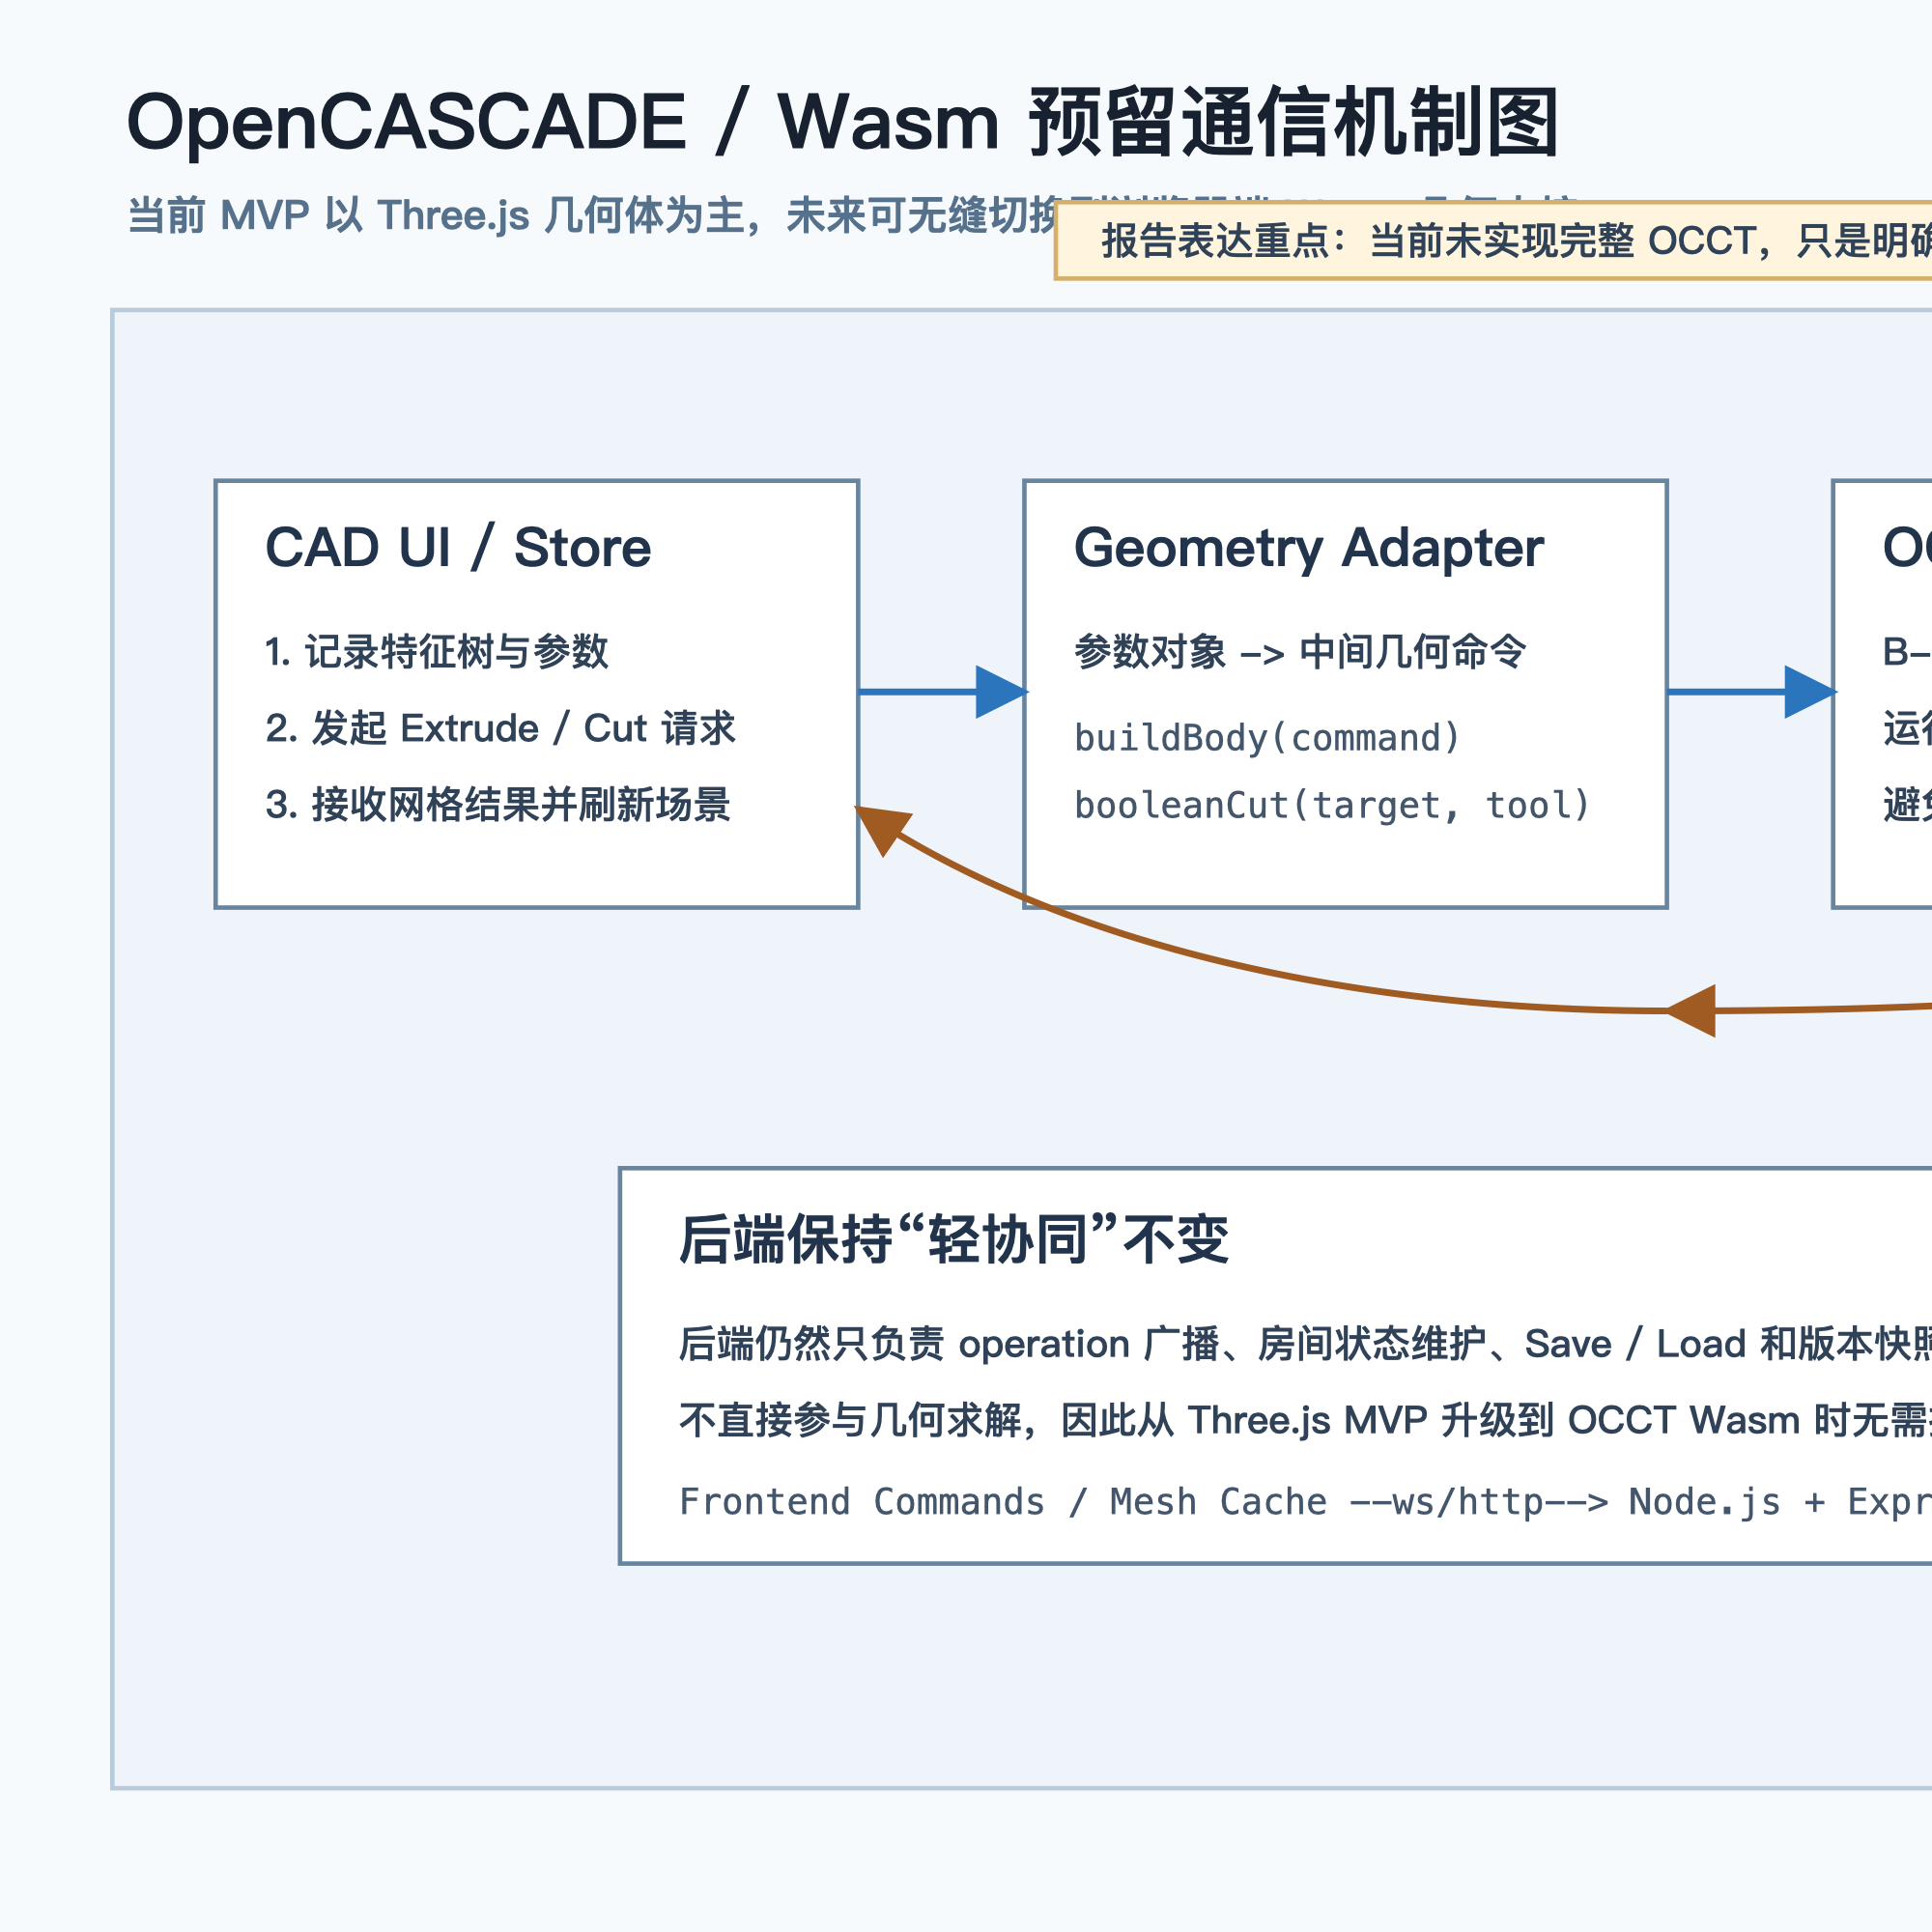
\includegraphics[width=\textwidth]{wasm-bridge.png}
\end{generalfig}

在该方案下：

\begin{itemize}[leftmargin=2em]
  \item Three.js 继续负责显示网格结果和交互；
  \item Wasm 模块负责复杂几何求解；
  \item 后端仍然只负责房间协同与持久化，不直接参与几何内核计算。
\end{itemize}

这种设计使当前 MVP 和未来工业级几何内核升级之间形成了清晰边界，也有助于在答辩时回答“为什么现在不用 OpenCASCADE、以后如何升级”的问题。

\section{关键功能实现}

\subsection{CAD 主界面}

系统主界面采用典型三栏 CAD 布局：顶部为 Ribbon 风格工具栏，左侧为 Feature Tree，中间为 Three.js 三维视图，右侧为属性面板，底部为状态栏。这种布局符合传统 CAD 操作认知，也便于演示。

\begin{generalfig}[htb]{系统主界面与建模视图}{fig:workspace}
  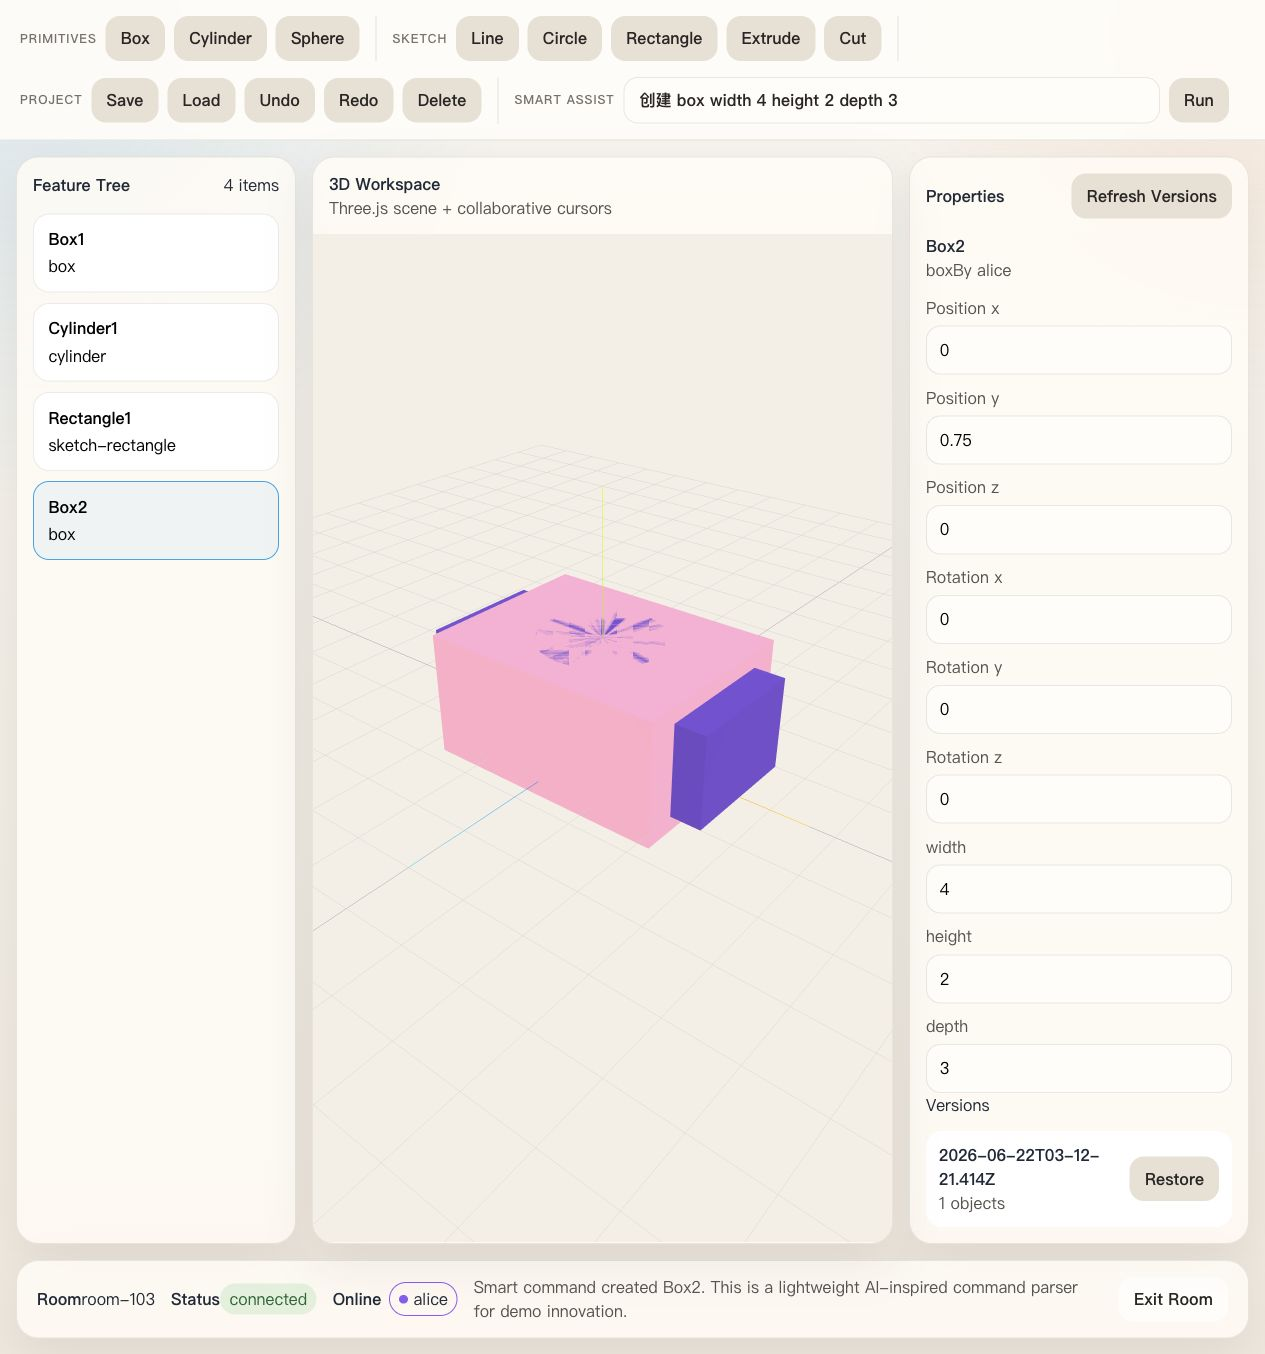
\includegraphics[width=\textwidth]{cad-workspace-demo.png}
\end{generalfig}

如\autoref{fig:workspace}所示，系统主界面能够同时展示对象树、三维模型、参数区和版本区，适合在答辩时完成完整功能链路演示。

\subsection{基础建模功能}

\subsubsection{基础实体}

系统支持三种基础实体：

\begin{itemize}[leftmargin=2em]
  \item Box：通过 \texttt{THREE.BoxGeometry} 实现；
  \item Cylinder：通过 \texttt{THREE.CylinderGeometry} 实现；
  \item Sphere：通过 \texttt{THREE.SphereGeometry} 实现。
\end{itemize}

\subsubsection{草图对象}

系统支持三种草图对象：

\begin{itemize}[leftmargin=2em]
  \item Line；
  \item Circle；
  \item Rectangle。
\end{itemize}

草图对象当前主要用于表达二维轮廓和为 Extrude 提供输入。

\subsubsection{Extrude}

当用户选中 Rectangle 或 Circle 草图后，可执行 Extrude。前端根据草图参数构造 \texttt{THREE.Shape}，再通过 \texttt{THREE.ExtrudeGeometry} 生成三维实体，完成从二维草图到三维模型的转化。

\subsubsection{Cut 的简化实现}

由于工业级布尔运算需要更强的几何内核支持，本系统没有实现完整实体差集，而是使用“切除区域可视化标记”的方式作为演示级简化实现。该处理在文档与答辩中已被明确说明为工程取舍。

\subsection{协同机制实现}

\subsubsection{房间机制}

系统以 \texttt{roomId} 作为协同作用域。多个用户进入同一个 \texttt{roomId} 后，共享同一份房间状态。

\subsubsection{操作广播}

后端通过 WebSocket 广播以下操作：

\begin{itemize}[leftmargin=2em]
  \item \texttt{add}
  \item \texttt{update}
  \item \texttt{delete}
  \item \texttt{replace-state}
  \item \texttt{cursor}
\end{itemize}

\subsubsection{冲突处理}

当前版本采用“最后写入优先（Last Write Wins）”策略。也就是后端按最新收到的操作覆盖对象状态。该策略实现简单，能很好满足课程设计中的双窗口协同演示。

\subsection{保存、加载与版本管理}

每次点击 Save 时，系统会执行两项操作：

\begin{enumerate}[leftmargin=2em]
  \item 更新当前房间主文件：\texttt{backend/data/projects/\{roomId\}.json}；
  \item 生成版本快照文件：
  \begin{flushleft}
    \texttt{backend/data/projects/\{roomId\}/versions/\{timestamp\}.json}
  \end{flushleft}
\end{enumerate}

同时系统支持：

\begin{itemize}[leftmargin=2em]
  \item Load：恢复最近一次保存状态；
  \item Restore：恢复指定历史版本；
  \item Undo / Redo：客户端本地历史回退与重做。
\end{itemize}

\subsection{Smart Assist 智能辅助建模}

为增强系统创新性，系统增加了 Smart Assist 命令入口。用户可输入：

\begin{quote}
创建 box width 4 height 2 depth 3
\end{quote}

系统通过轻量规则解析器识别对象类型与参数，并自动生成对应对象。该实现无需依赖外部大模型，但体现了“自然语言驱动 CAD 操作”的交互方向，也为后续接入 AI 模型保留了扩展位。

\section{测试与结果分析}

\subsection{测试矩阵}

为验证系统覆盖课程设计要求，本文设计了测试矩阵，如\autoref{tab:testmatrix}所示。

\begin{generaltab}{系统测试矩阵与考核映射}{tab:testmatrix}
\begin{tabularx}{\textwidth}{l l X l}
\toprule
测试编号 & 测试项 & 预期结果 & 对应考核项 \\
\midrule
T1 & 前后端启动 & backend 与 frontend 均可正常运行 & 核心功能、代码质量 \\
T3 & Box / Cylinder 建模 & 对象树与场景中正确出现实体 & 核心功能实现 \\
T6 & Extrude & 从草图生成三维实体 & 核心功能实现 \\
T8 & 双窗口协同 & 另一窗口实时看到同步结果 & 核心功能、演示答辩 \\
T10 & Save / Load & 最近保存状态可恢复 & 核心功能实现 \\
T12 & 版本恢复 & 指定历史版本可恢复 & 核心功能实现 \\
T13 & Undo / Redo & 对象状态能回退与重做 & 核心功能实现 \\
T14 & Smart Assist & 自动创建对应对象 & 创新性 \\
\bottomrule
\end{tabularx}
\end{generaltab}

\subsection{验证结果}

当前系统已经获得如下验证证据：

\begin{itemize}[leftmargin=2em]
  \item 前端构建通过：\texttt{npm run build}；
  \item 后端类型检查通过：\texttt{npm run typecheck}；
  \item 双窗口房间协同、新建对象同步、属性同步、保存与版本恢复已经完成联调验证；
  \item Extrude、Undo / Redo 与 Smart Assist 已通过自动化脚本完成页面级验收；
  \item 已生成系统主界面截图与考核标准对照图；
  \item 代码与文档已同步到 GitHub 仓库。
\end{itemize}

\begin{generalfig}[htb]{双窗口实时协同验收图}{fig:collabproof}
  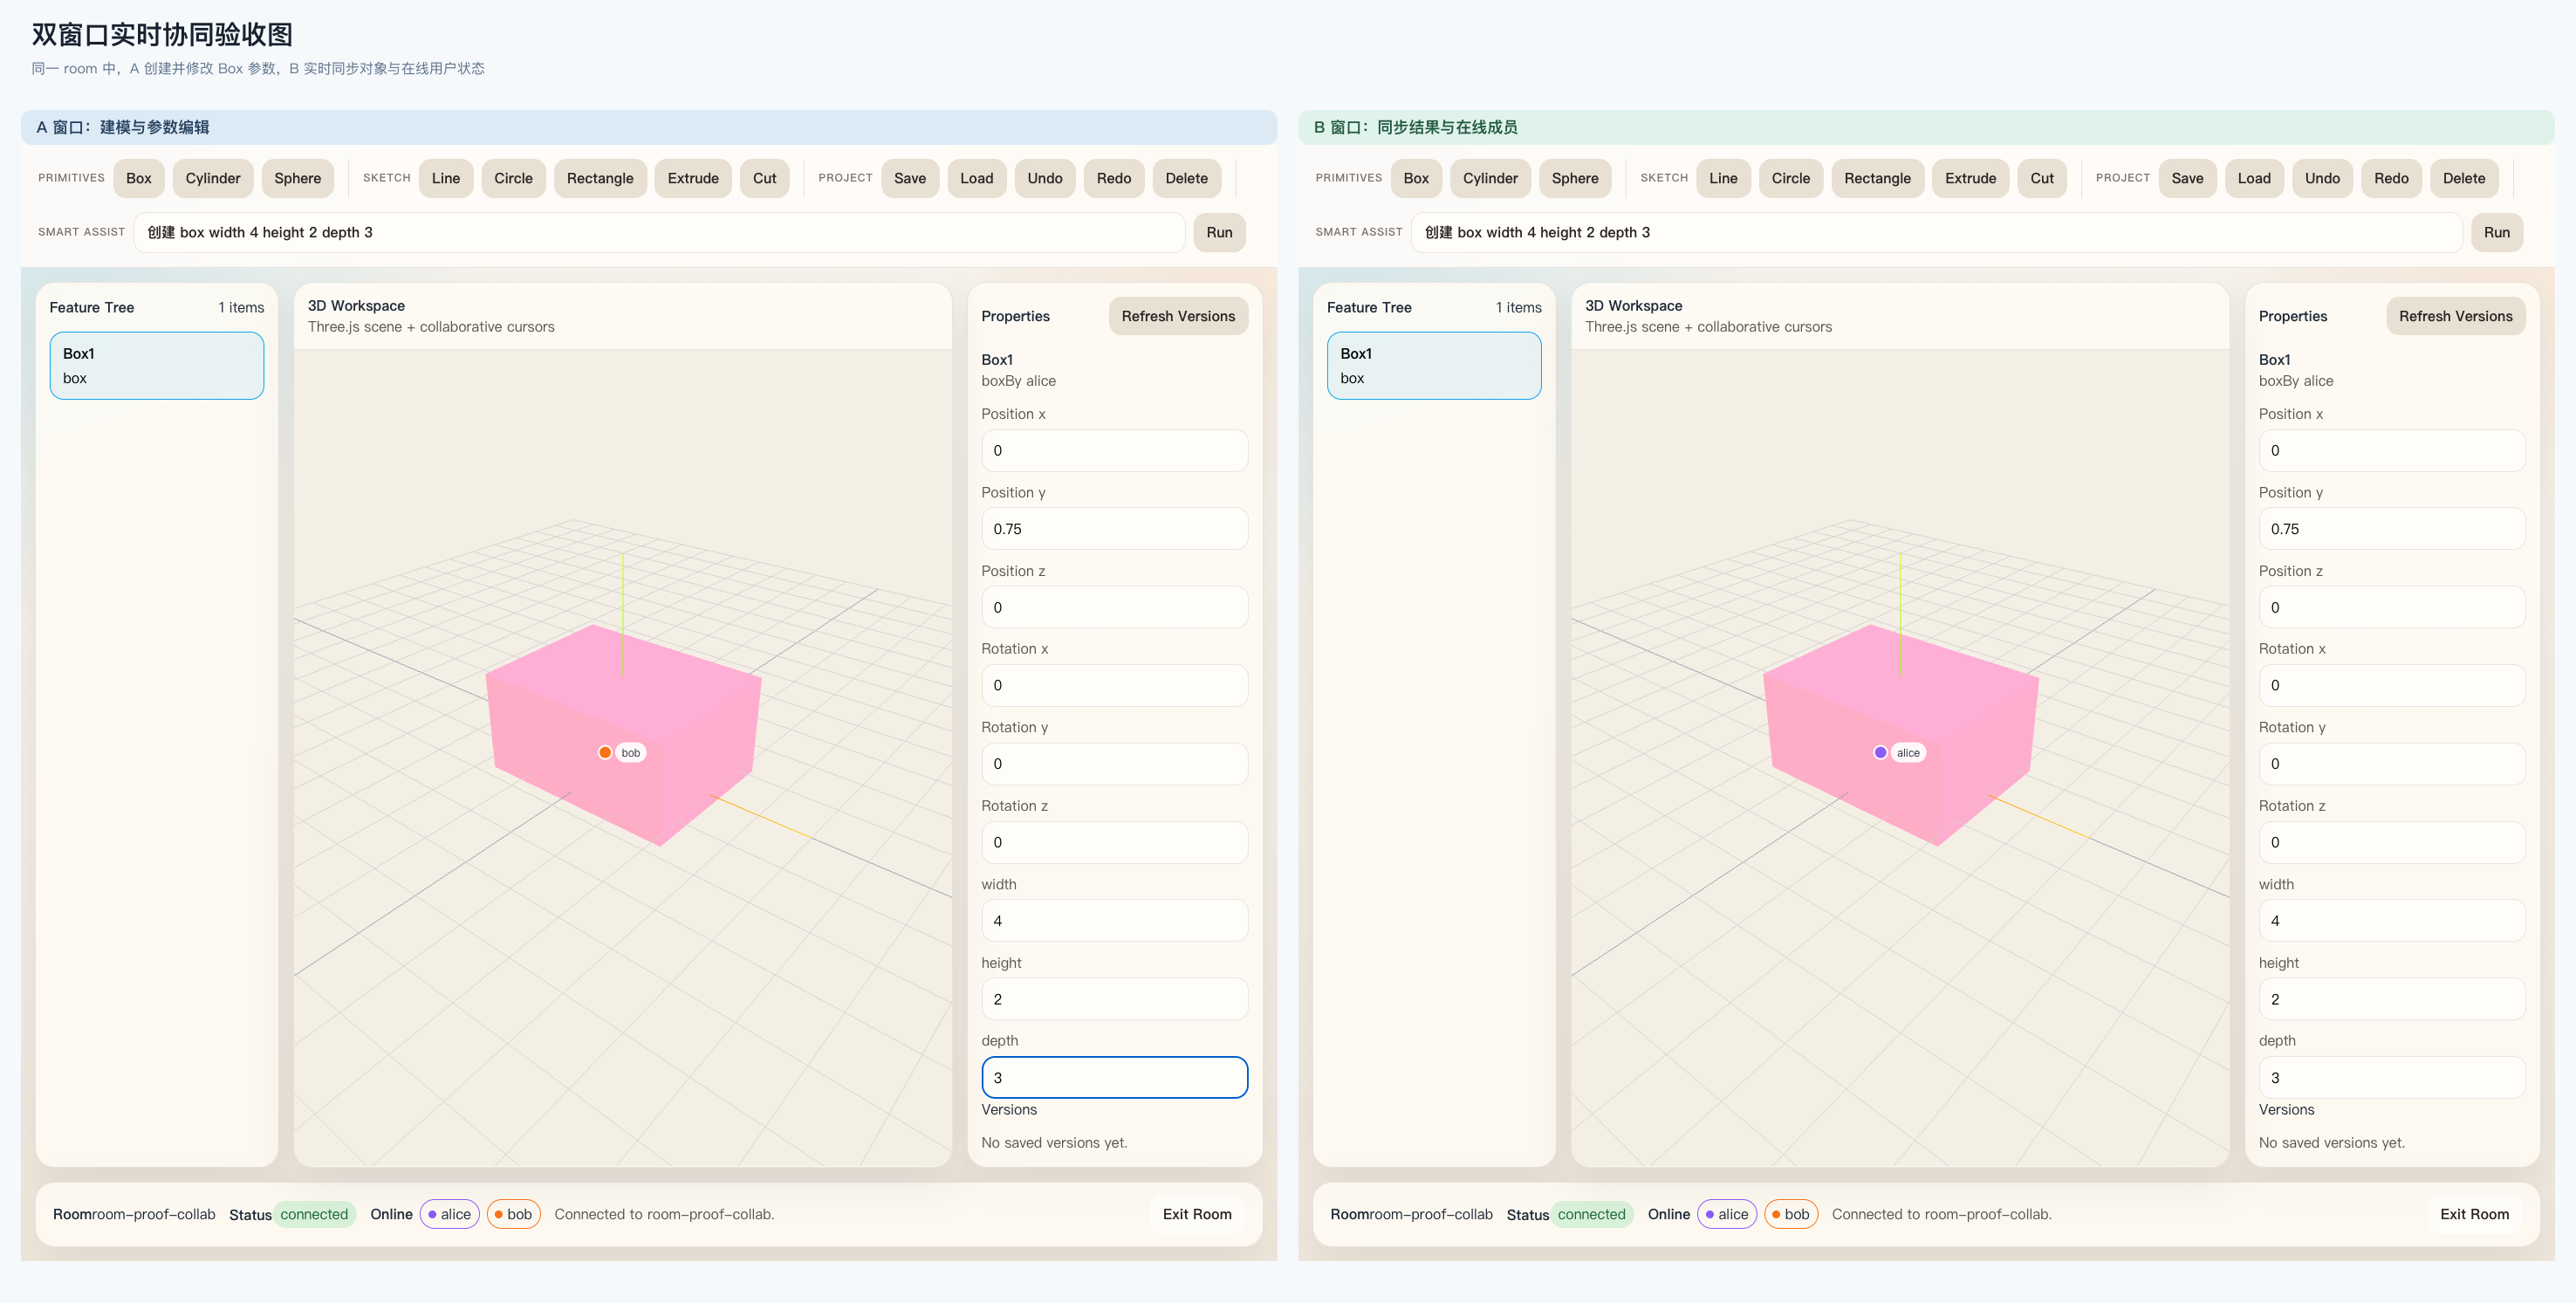
\includegraphics[width=\textwidth]{collab-sync-proof.png}
\end{generalfig}

\begin{generalfig}[htb]{保存与版本快照验收图}{fig:versionproof}
  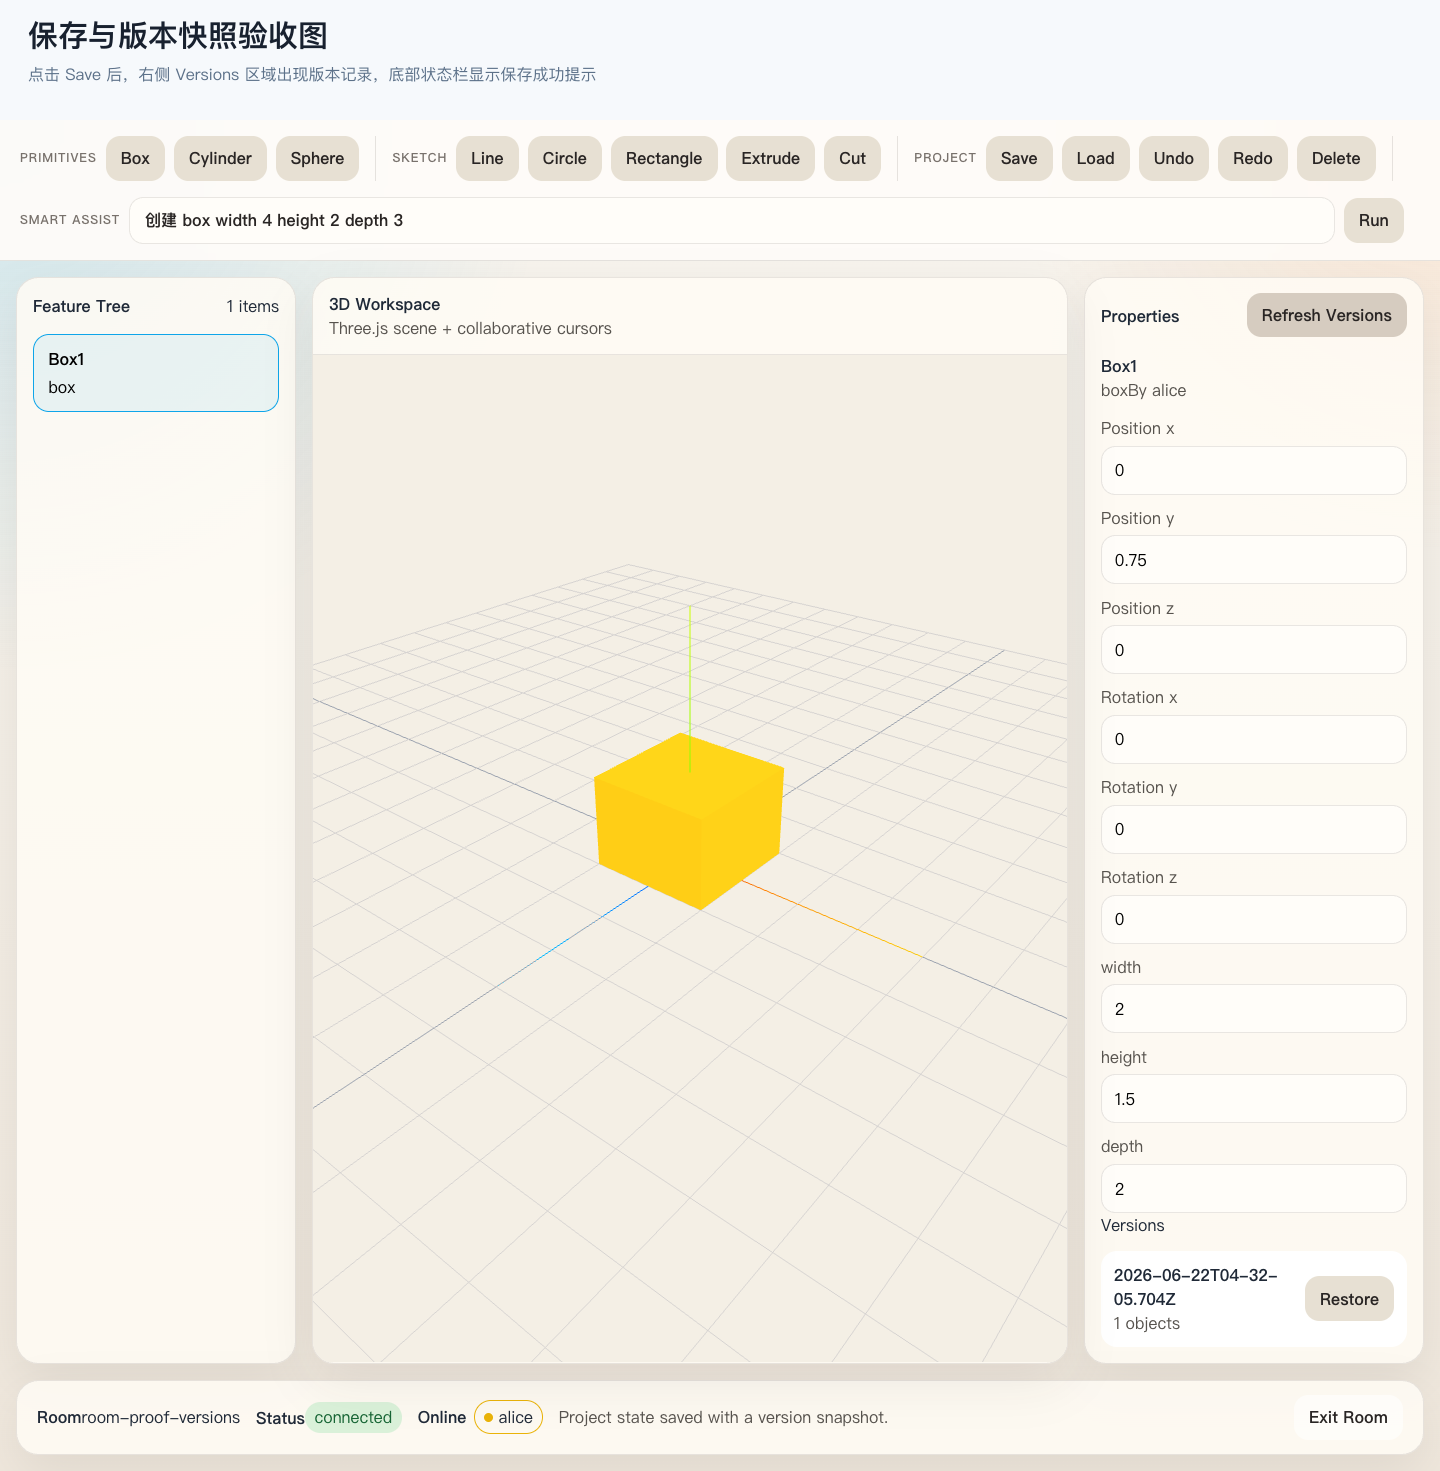
\includegraphics[width=\textwidth]{version-proof.png}
\end{generalfig}

\begin{generalfig}[htb]{Extrude 功能验收图}{fig:extrudeproof}
  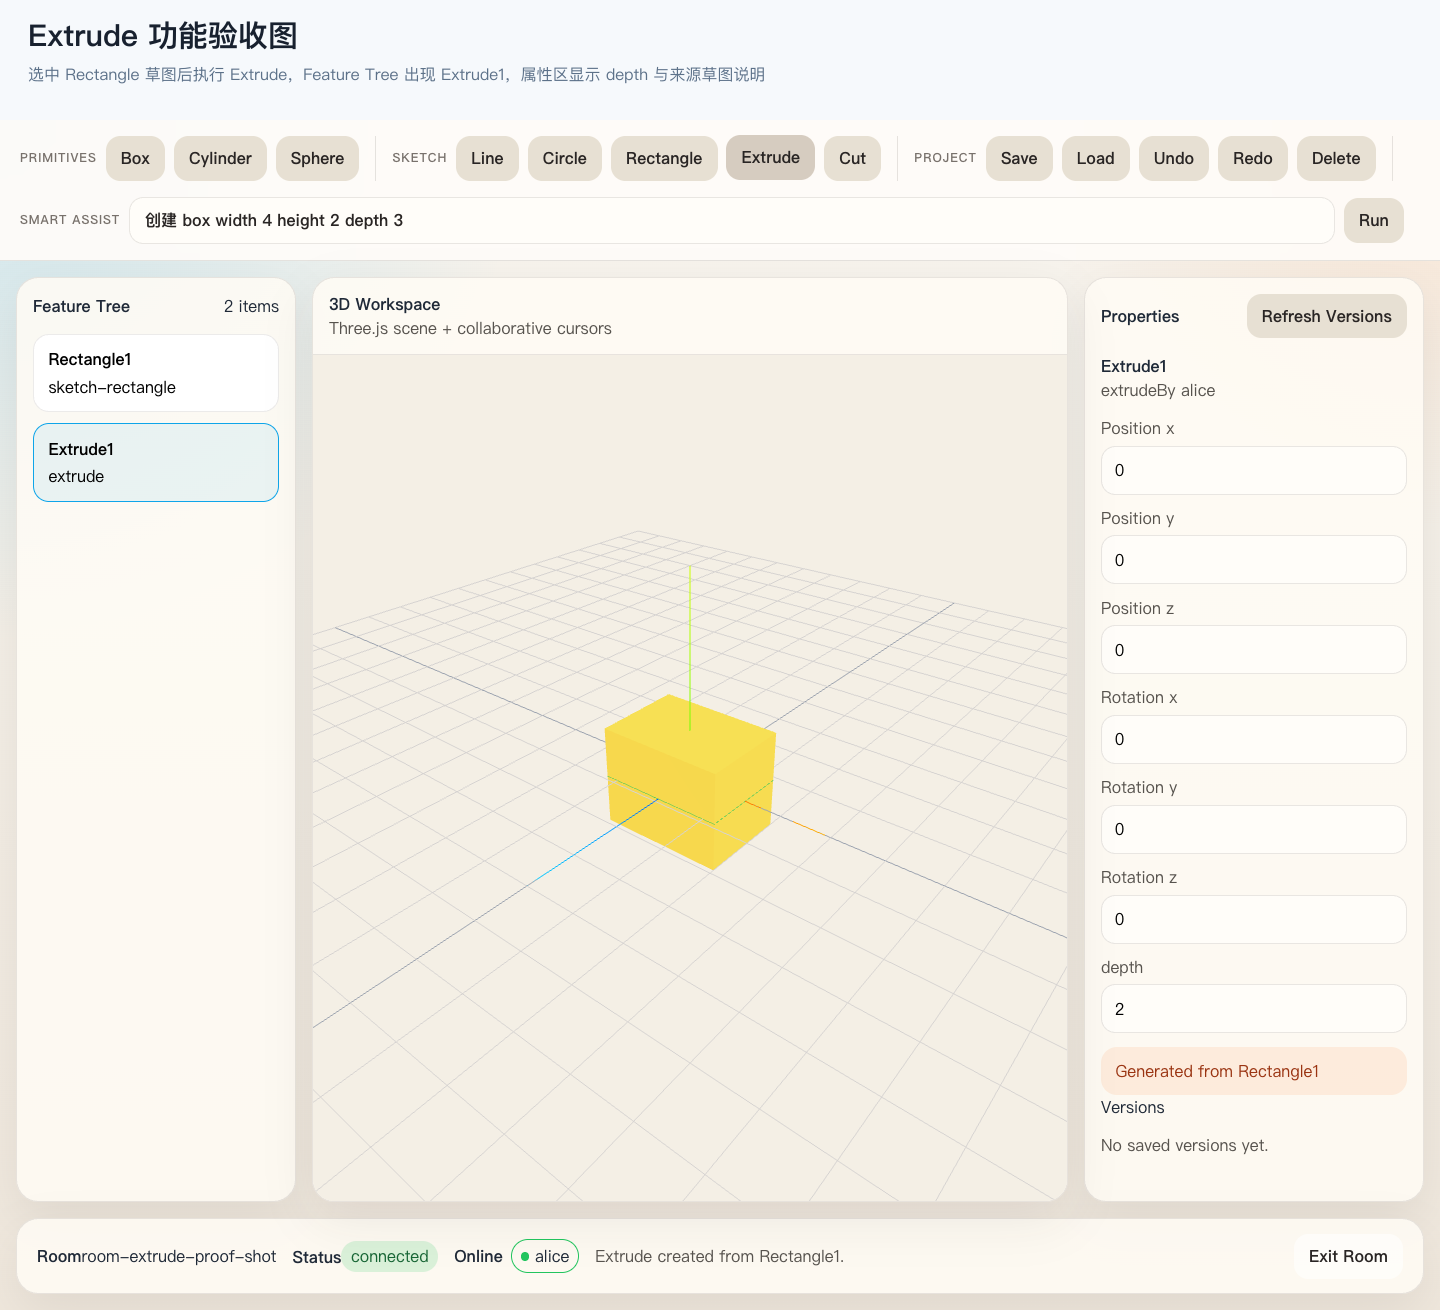
\includegraphics[width=\textwidth]{extrude-proof.png}
\end{generalfig}

\begin{generalfig}[htb]{Undo / Redo 功能验收图}{fig:undoproof}
  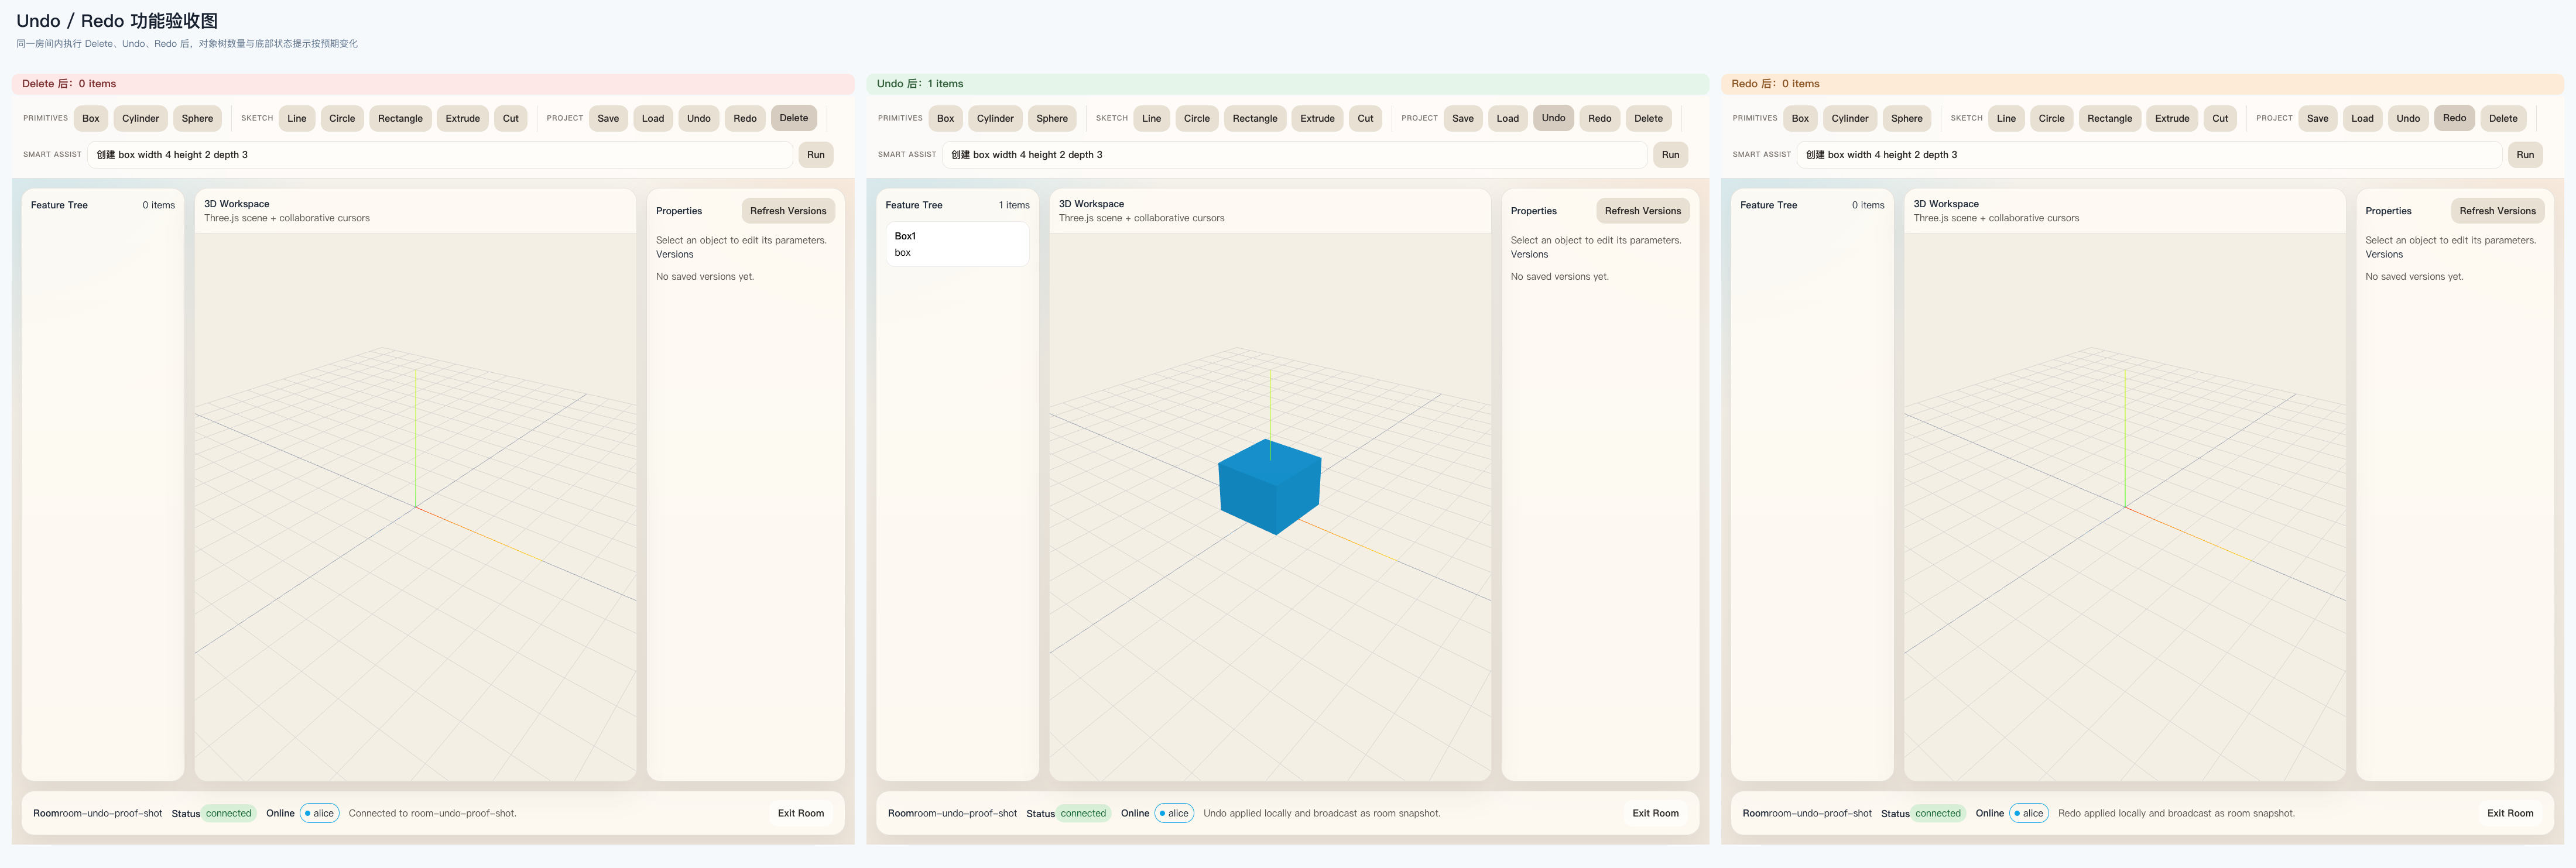
\includegraphics[width=\textwidth]{undo-redo-proof.png}
\end{generalfig}

\begin{generalfig}[htb]{Smart Assist 功能验收图}{fig:smartproof}
  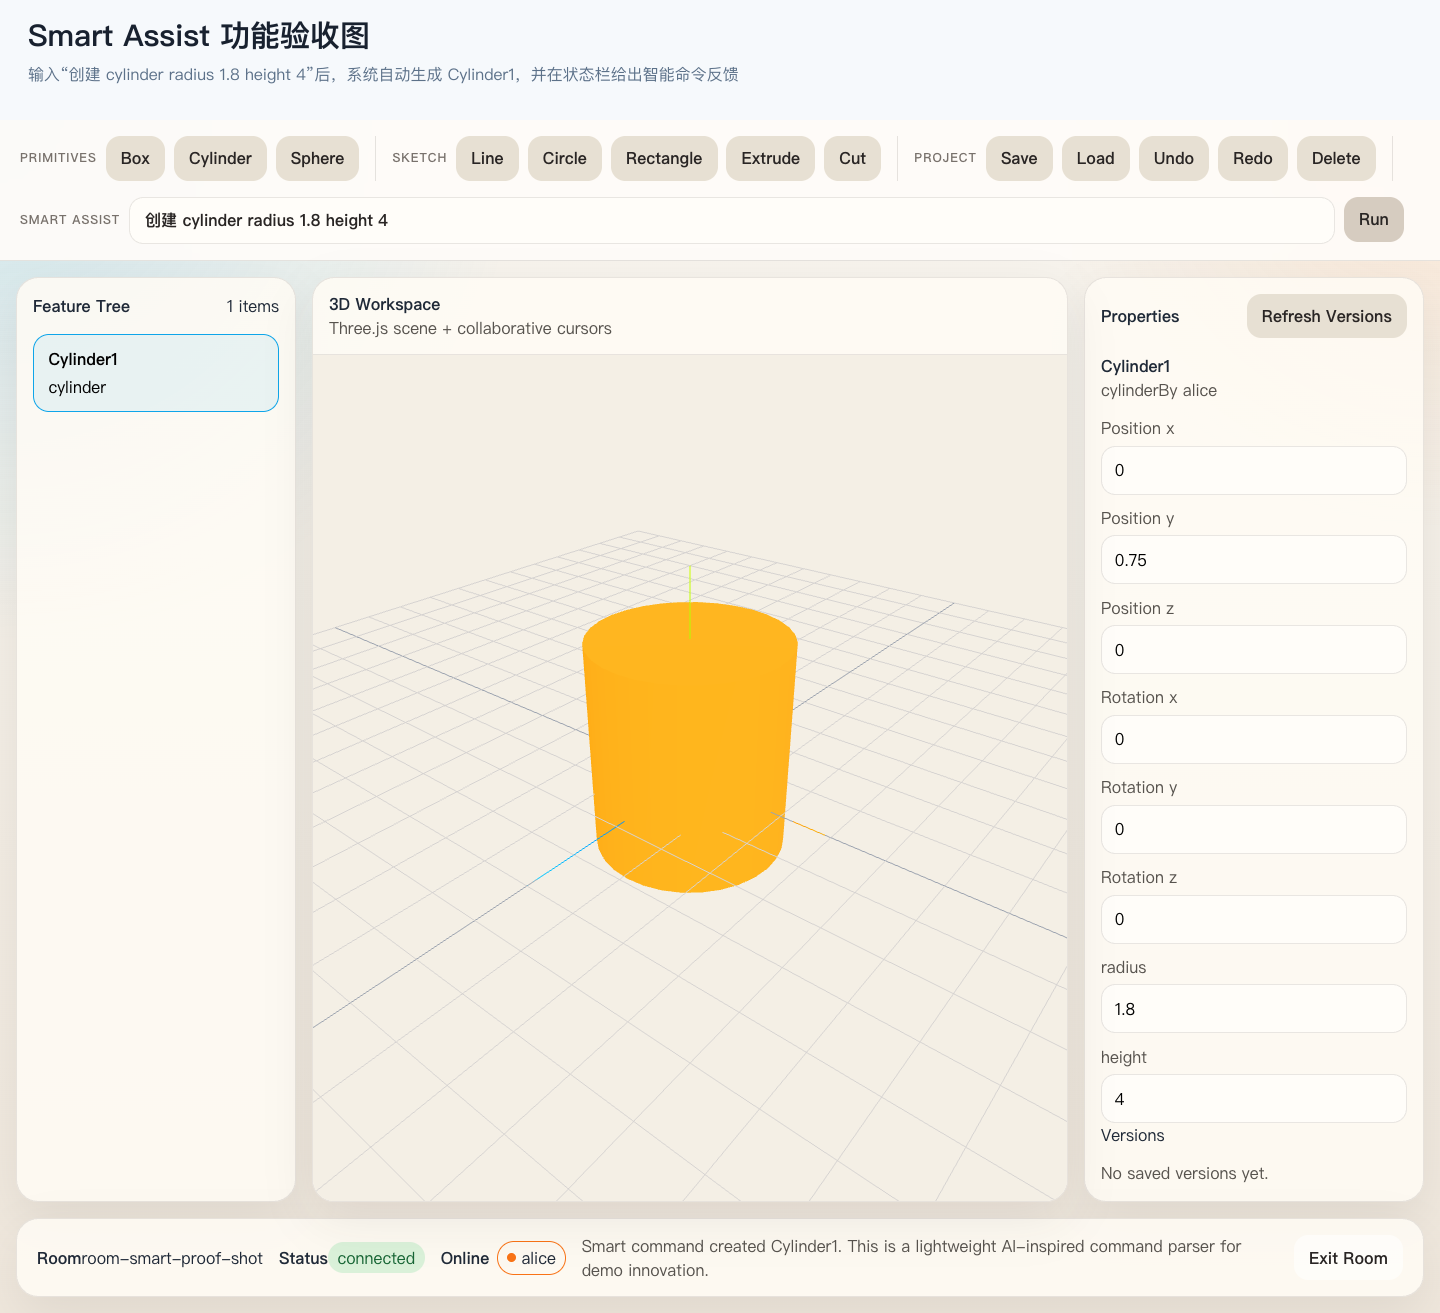
\includegraphics[width=\textwidth]{smart-assist-proof.png}
\end{generalfig}

\begin{generalfig}[htb]{考核标准对照图}{fig:scorecard}
  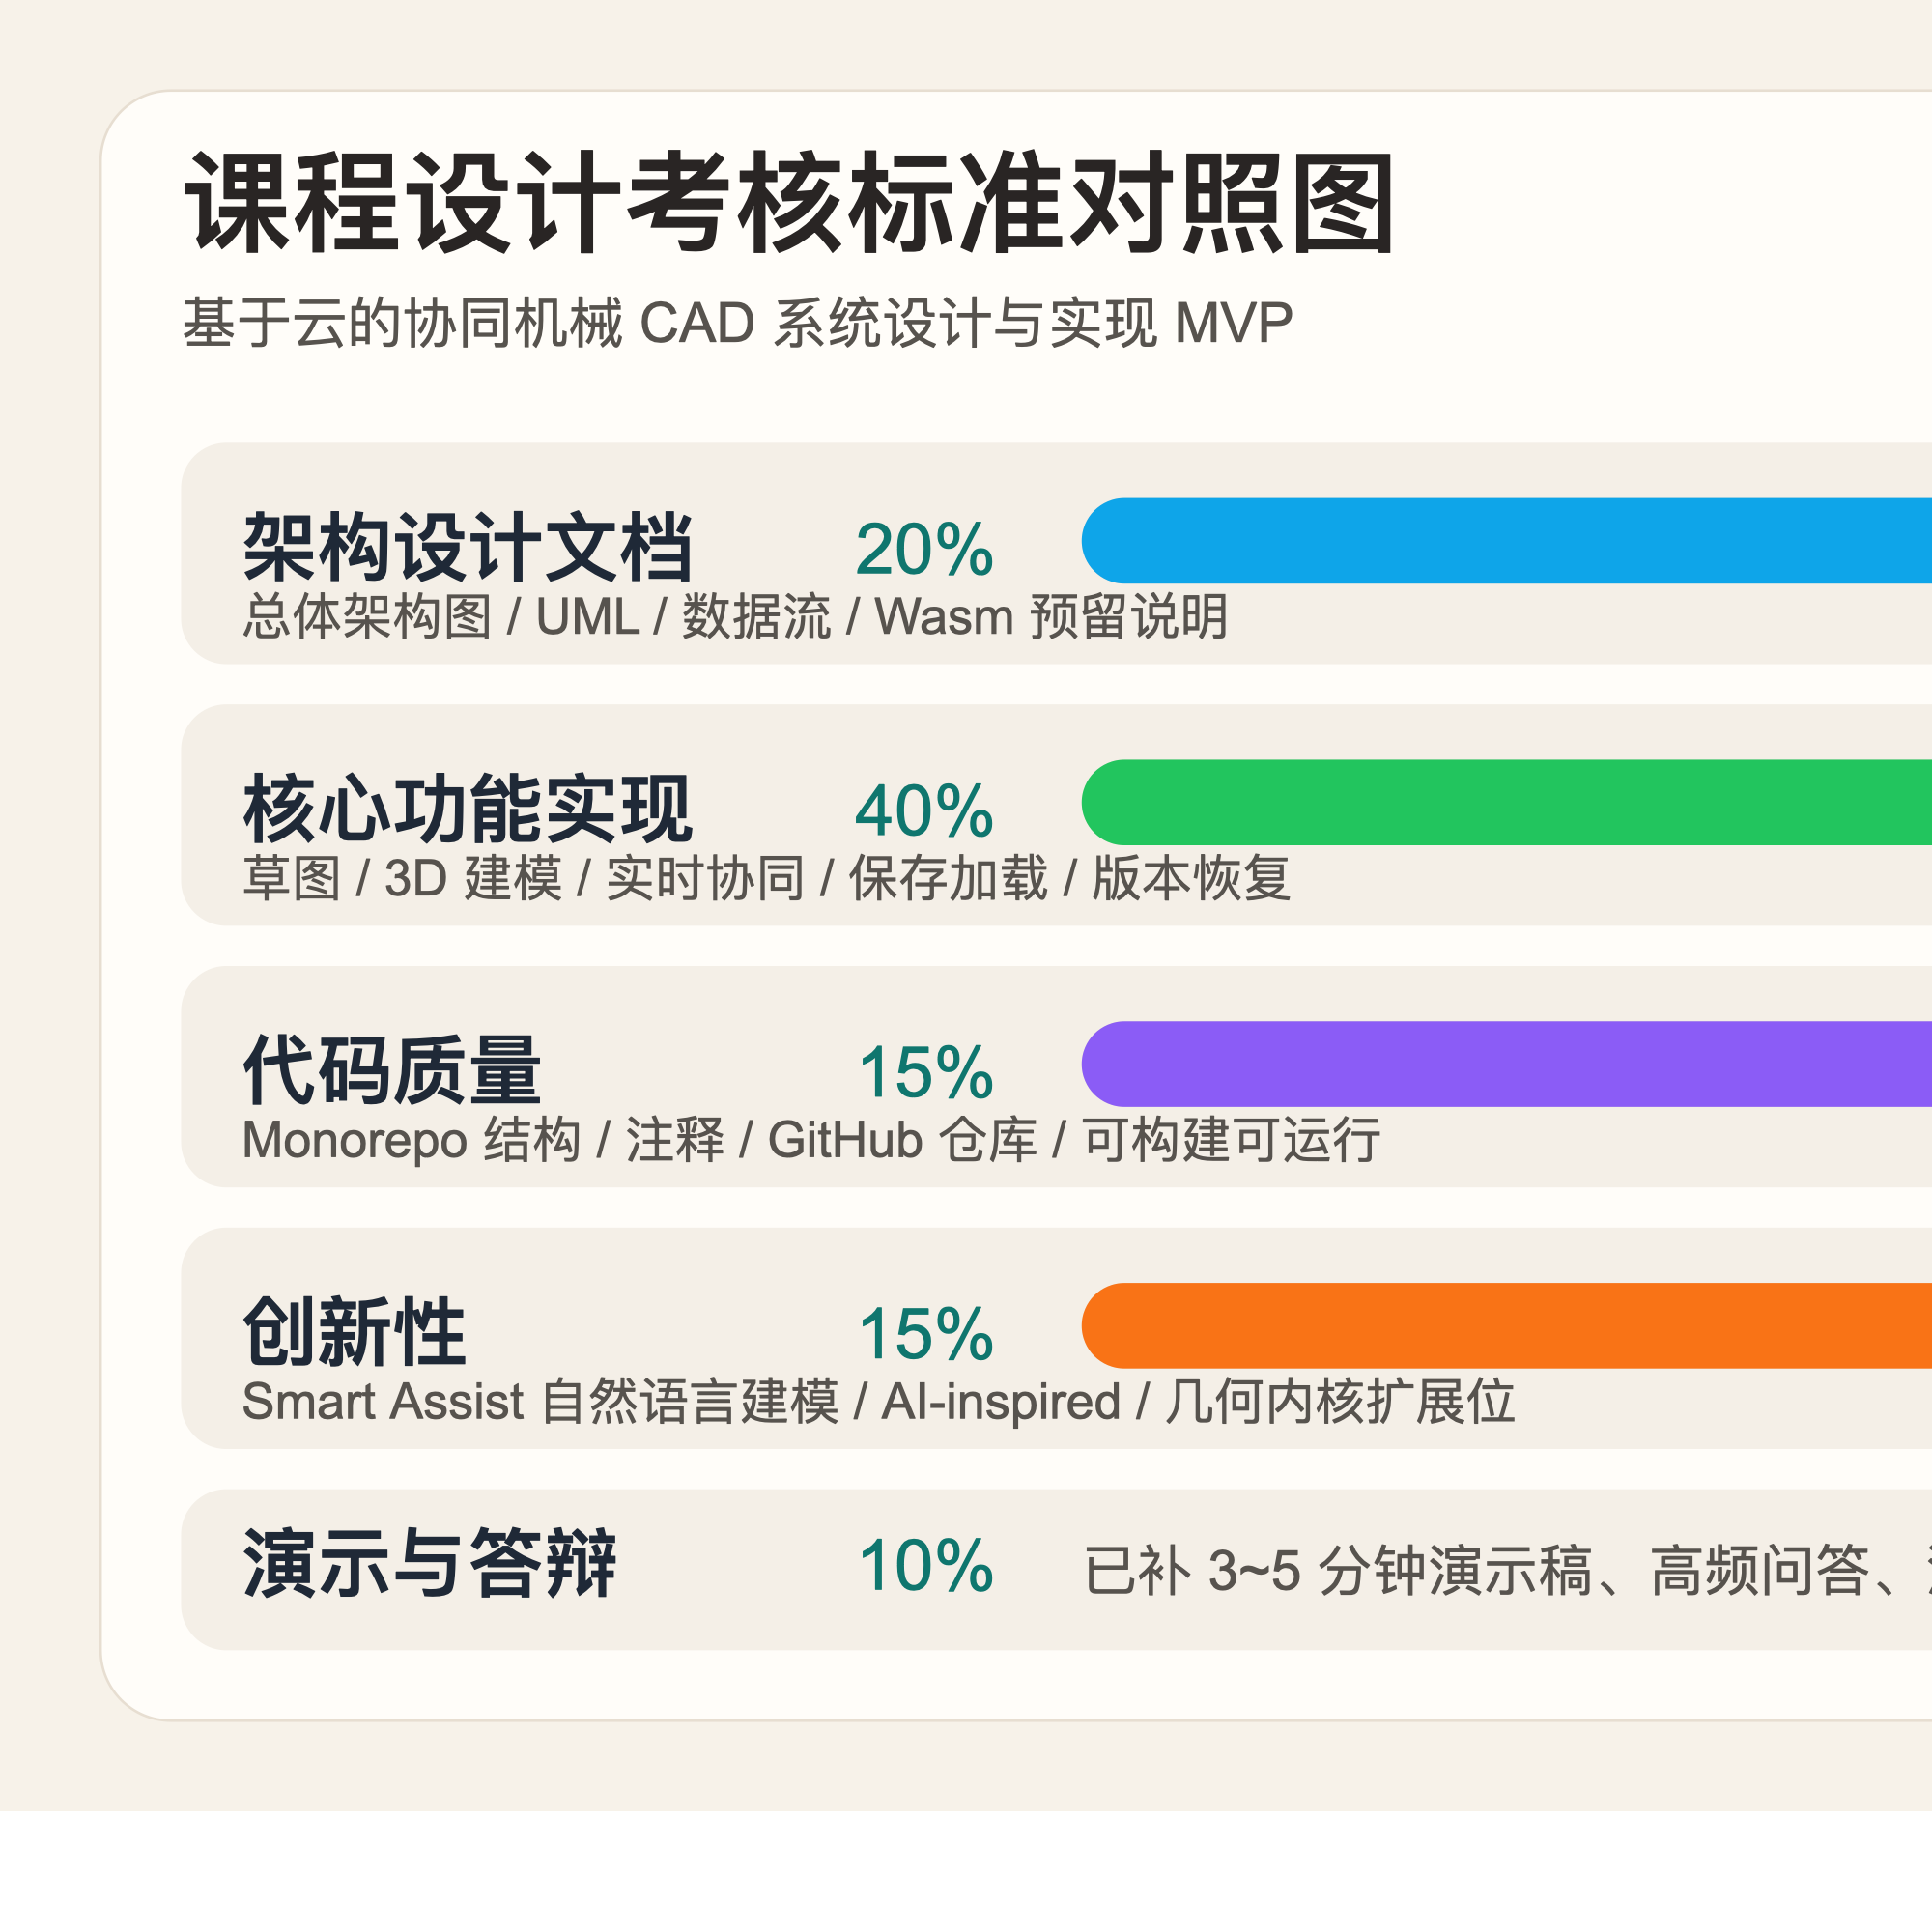
\includegraphics[width=\textwidth]{evaluation-scorecard.png}
\end{generalfig}

如\autoref{fig:scorecard}所示，系统已经围绕架构设计文档、核心功能实现、代码质量、创新性和演示答辩五个评分项分别准备了对应材料。
其中，\autoref{fig:collabproof} 直接证明了同房间双窗口下对象创建、参数修改、远端光标和在线用户状态的同步效果；\autoref{fig:versionproof} 证明了 Save 后版本快照生成、版本列表刷新和后续 Restore 入口的可用性；\autoref{fig:extrudeproof}、\autoref{fig:undoproof} 与 \autoref{fig:smartproof} 则分别补足了拉伸建模、操作回退重做和智能辅助建模三项核心能力的可视化证据。

\subsection{结果分析}

综合实现与测试结果可以看出：

\begin{itemize}[leftmargin=2em]
  \item 系统完成了课程设计要求中的核心闭环；
  \item 系统结构清晰，便于答辩时按模块说明；
  \item 系统强调稳定演示而非复杂内核，是合理的工程取舍；
  \item Smart Assist 与 Wasm 扩展位增强了创新性叙事。
\end{itemize}

\section{创新点与工程取舍}

\subsection{创新点}

本项目的创新点主要体现在：

\begin{enumerate}[leftmargin=2em]
  \item 在较低复杂度下实现了云协同 CAD 的可运行 MVP；
  \item 采用前端重计算、后端轻协同的工程架构；
  \item 增加了 Smart Assist 自然语言辅助建模入口；
  \item 在架构中预留了 OpenCASCADE/Wasm、PostgreSQL、OBS 和 AI 辅助设计扩展位。
\end{enumerate}

\subsection{工程取舍}

为了保证课程设计交付目标，本项目做出了以下工程取舍：

\begin{itemize}[leftmargin=2em]
  \item 未集成工业级几何内核，而使用 Three.js 保证稳定性；
  \item 未实现完整布尔差，而采用简化 Cut 可视化；
  \item 未引入数据库，而采用本地 JSON 降低部署成本；
  \item 未依赖外部 AI 服务，而采用规则型智能辅助入口。
\end{itemize}

\section{总结与展望}

本文完成了一个基于云协同思想的机械 CAD 系统 MVP 的设计与实现。系统在课程设计范围内实现了基础建模、草图表达、拉伸成型、实时协同、保存加载、版本管理以及轻量智能辅助建模等关键功能，并围绕考核标准进一步形成了架构图示、测试矩阵、验收截图和课程报告等配套材料。

本项目的主要价值在于：在不追求工业级几何内核完整实现的前提下，通过合理的技术选型与工程取舍，完成了一个结构清晰、演示稳定、功能闭环完整且便于后续扩展的云协同 CAD 课程设计作品。该实现既满足了课程考核中“能运行、能展示、能说明”的基本要求，也为后续向更高保真度的 Web CAD 系统演进保留了明确接口边界。

后续工作可进一步从以下方面展开：

\begin{itemize}[leftmargin=2em]
  \item 接入 OpenCASCADE/Wasm，提升几何建模能力；
  \item 引入 PostgreSQL 与 OBS，实现更完整的云端存储；
  \item 增加 JWT 登录与权限控制；
  \item 引入大模型，实现更强的自然语言建模与参数推荐。
\end{itemize}

\bibliography{references}

\signature[blank lines=12em]

\end{document}
